%%%%%%%%%%%%%%%%%%%%%%%%%%%%%%%%%%%%%%%%%%%%%%%%%%%%%%%%%%%%%%%%%%%%%%
% Overleaf (WriteLaTeX) Example: Molecular Chemistry Presentation
%
% Source: http://www.overleaf.com
%
% In these slides we show how Overleaf can be used with standard 
% chemistry packages to easily create professional presentations.
% 
% Feel free to distribute this example, but please keep the referral
% to overleaf.com
% 
%%%%%%%%%%%%%%%%%%%%%%%%%%%%%%%%%%%%%%%%%%%%%%%%%%%%%%%%%%%%%%%%%%%%%%

\documentclass[xcolor={dvipsnames}]{beamer}

\mode<presentation>
{
  \usetheme{Madrid}       % or try default, Darmstadt, Warsaw, ...
  \usecolortheme{default} % or try albatross, beaver, crane, ...
  \usefonttheme{default}    % or try default, structurebold, ...
  \setbeamertemplate{navigation symbols}{}
  \setbeamertemplate{caption}[numbered]
} 

\usepackage[english]{babel}
\usepackage[utf8x]{inputenc}
\usepackage{graphicx}
\usepackage{hyperref}
  \hypersetup{colorlinks=true}
  \hypersetup{urlcolor=blue}
  \hypersetup{linkcolor = .}
\usepackage{xcolor}
\usepackage{siunitx}
  \sisetup{separate-uncertainty = true}
\usepackage{physics}
\usepackage[font=small,labelfont=bf]{caption}
\usepackage{subcaption}
\usepackage[en-GB]{datetime2}
\usepackage{overpic}
\usepackage{feynmp}
\DeclareGraphicsRule{*}{mps}{*}{}
\usepackage{scalerel}
\newcommand{\mylbrace}[2]{\vspace{#2pt}\hspace{6pt}\scaleleftright[\dimexpr5pt+#1\dimexpr0.06pt]{\lbrace}{\rule[\dimexpr2pt-#1\dimexpr0.5pt]{-4pt}{#1pt}}{.}}
\newcommand{\myrbrace}[2]{\vspace{#2pt}\scaleleftright[\dimexpr5pt+#1\dimexpr0.06pt]{.}{\rule[\dimexpr2pt-#1\dimexpr0.5pt]{-4pt}{#1pt}}{\rbrace}\hspace{6pt}}

% Trim in percent
\usepackage{adjustbox}

% No "Figure" prefix
\setbeamertemplate{caption}{\raggedright\insertcaption\par}

% Nice decay amplitude diagrams
\usepackage{amsmath,amssymb,tikz-cd}

% Strike out text
\usepackage[normalem]{ulem}

% For figures with text overlay
\usepackage{overpic}

% Arrows
\usepackage{tikz}
\newcommand{\tikzmark}[1]{\tikz[remember picture] \node[coordinate] (#1) {#1};}

% Colourbox with line breaks
\newcommand{\cbox}[2][lime!20]{%
  \colorbox{#1}{\parbox{\dimexpr\linewidth-2\fboxsep}{\strut #2\strut}}%
}

% Vector arrows
\usepackage[pdftex]{pict2e}

% Here's where the presentation starts, with the info for the title slide
\title[Beauty 2023]{Measurements of CKM angle \texorpdfstring{$\gamma$}{gamma} in LHCb}

\author[Martin Tat]{Martin Tat, on behalf of the LHCb collaboration}
\institute[University of Oxford]{\normalsize University of Oxford\\ \vspace{0.3cm}\normalsize Beauty 2023, Clermont-Ferrand}
\date{3rd-7th July 2023}

\titlegraphic{
\includegraphics[height = 2.8cm]{lhcb.jpg}\hspace{1.5cm}~%
              
\includegraphics[height = 2.8cm]{OxfordLogo.pdf}}

\begin{document}

\begin{frame}
  \titlepage
\end{frame}

% These three lines create an automatically generated table of contents.
% \begin{frame}{Outline}
%   \tableofcontents
% \end{frame}

\section{Introduction to \texorpdfstring{$\gamma$}{gamma} and \texorpdfstring{$C\!P$}{CP} violation}
\begin{frame}{Introduction to $\gamma$ and $C\!P$ violation}
  \begin{itemize}
    \setlength\itemsep{0.3em}
    \item{CPV in SM is described by the Unitary Triangle, with angles $\alpha$, $\beta$, $\gamma$}
    \item{The angle $\gamma = \text{arg}\Big(-\frac{V^{\phantom{*}}_{ud}V^*_{ub}}{V^{\phantom{*}}_{cd}V^*_{cb}}\Big)$ is very important:}
    \begin{enumerate}
    \setlength\itemsep{0.2em}
      \item{Negligible theoretical uncertainties: Ideal SM benchmark}
      \item{Accessible at tree level: Indirectly probe New Physics that enter loops}
      \item{Compare with a global CKM fit: Is the Unitary Triangle a triangle?}
    \end{enumerate}
  \end{itemize}
  \vspace{-0.2cm}
  \begin{figure}
    \centering
    \begin{subfigure}{0.5\textwidth}
      \centering
      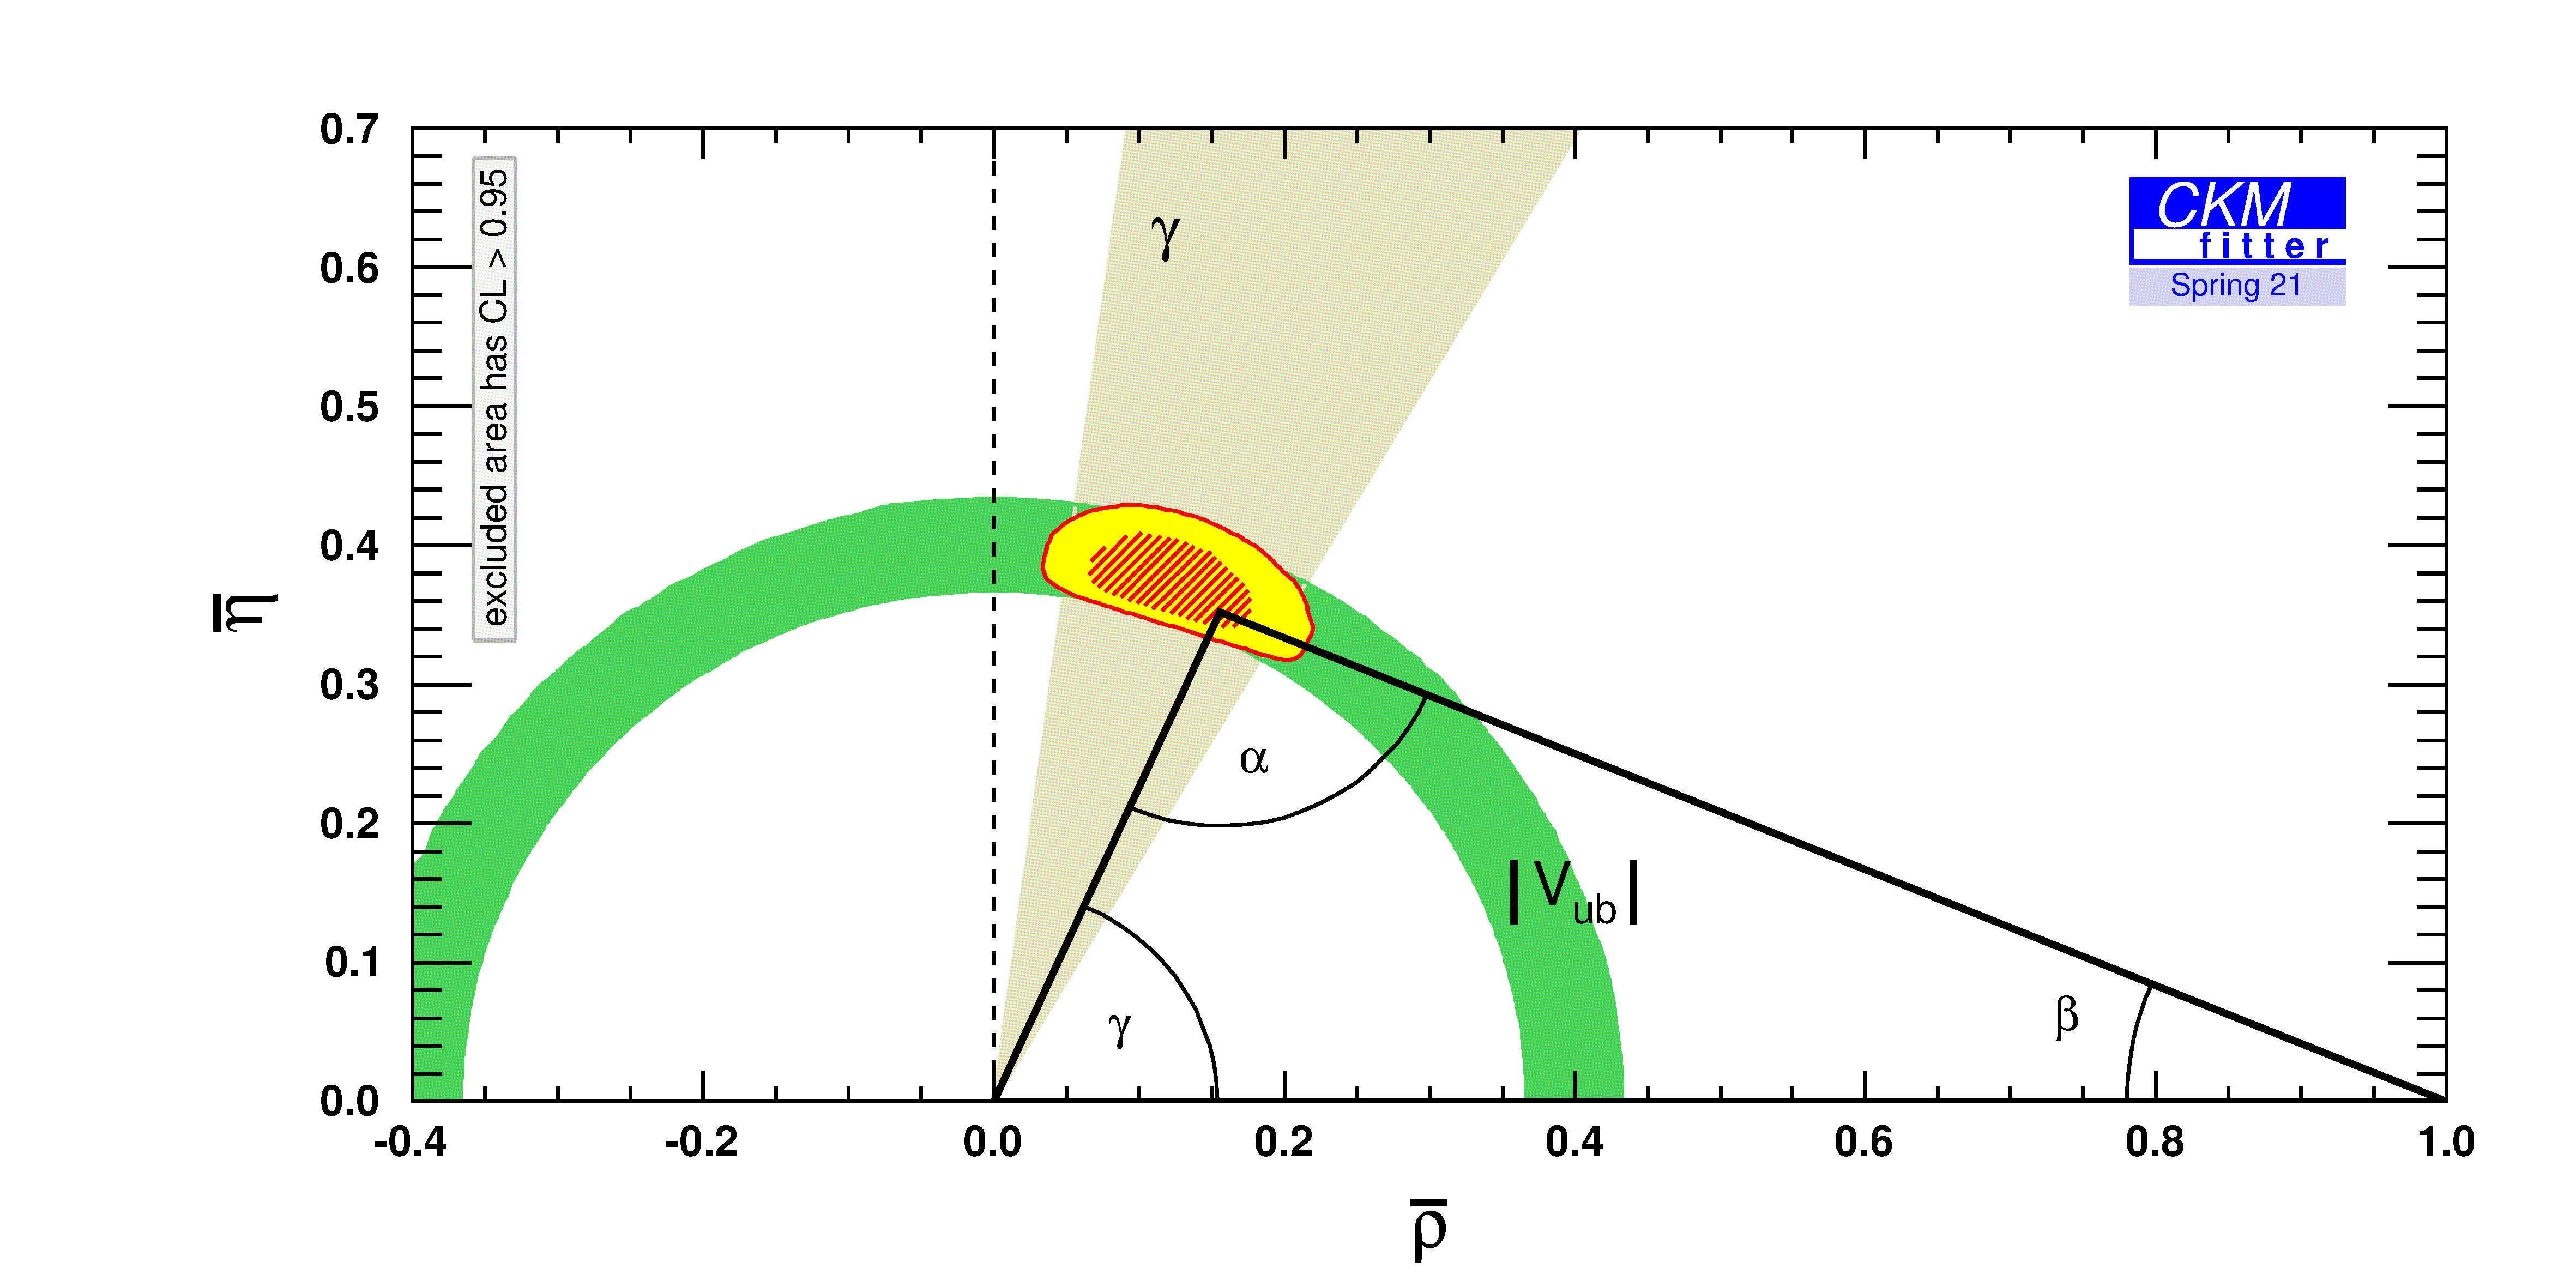
\includegraphics[width = 1.0\textwidth]{Plots/ckmfitter_tree.png}
      \caption{Tree level: $\gamma = \big(72.1^{+5.4}_{-5.7}\big)^\circ$}
    \end{subfigure}%
    \begin{subfigure}{0.5\textwidth}
      \centering
      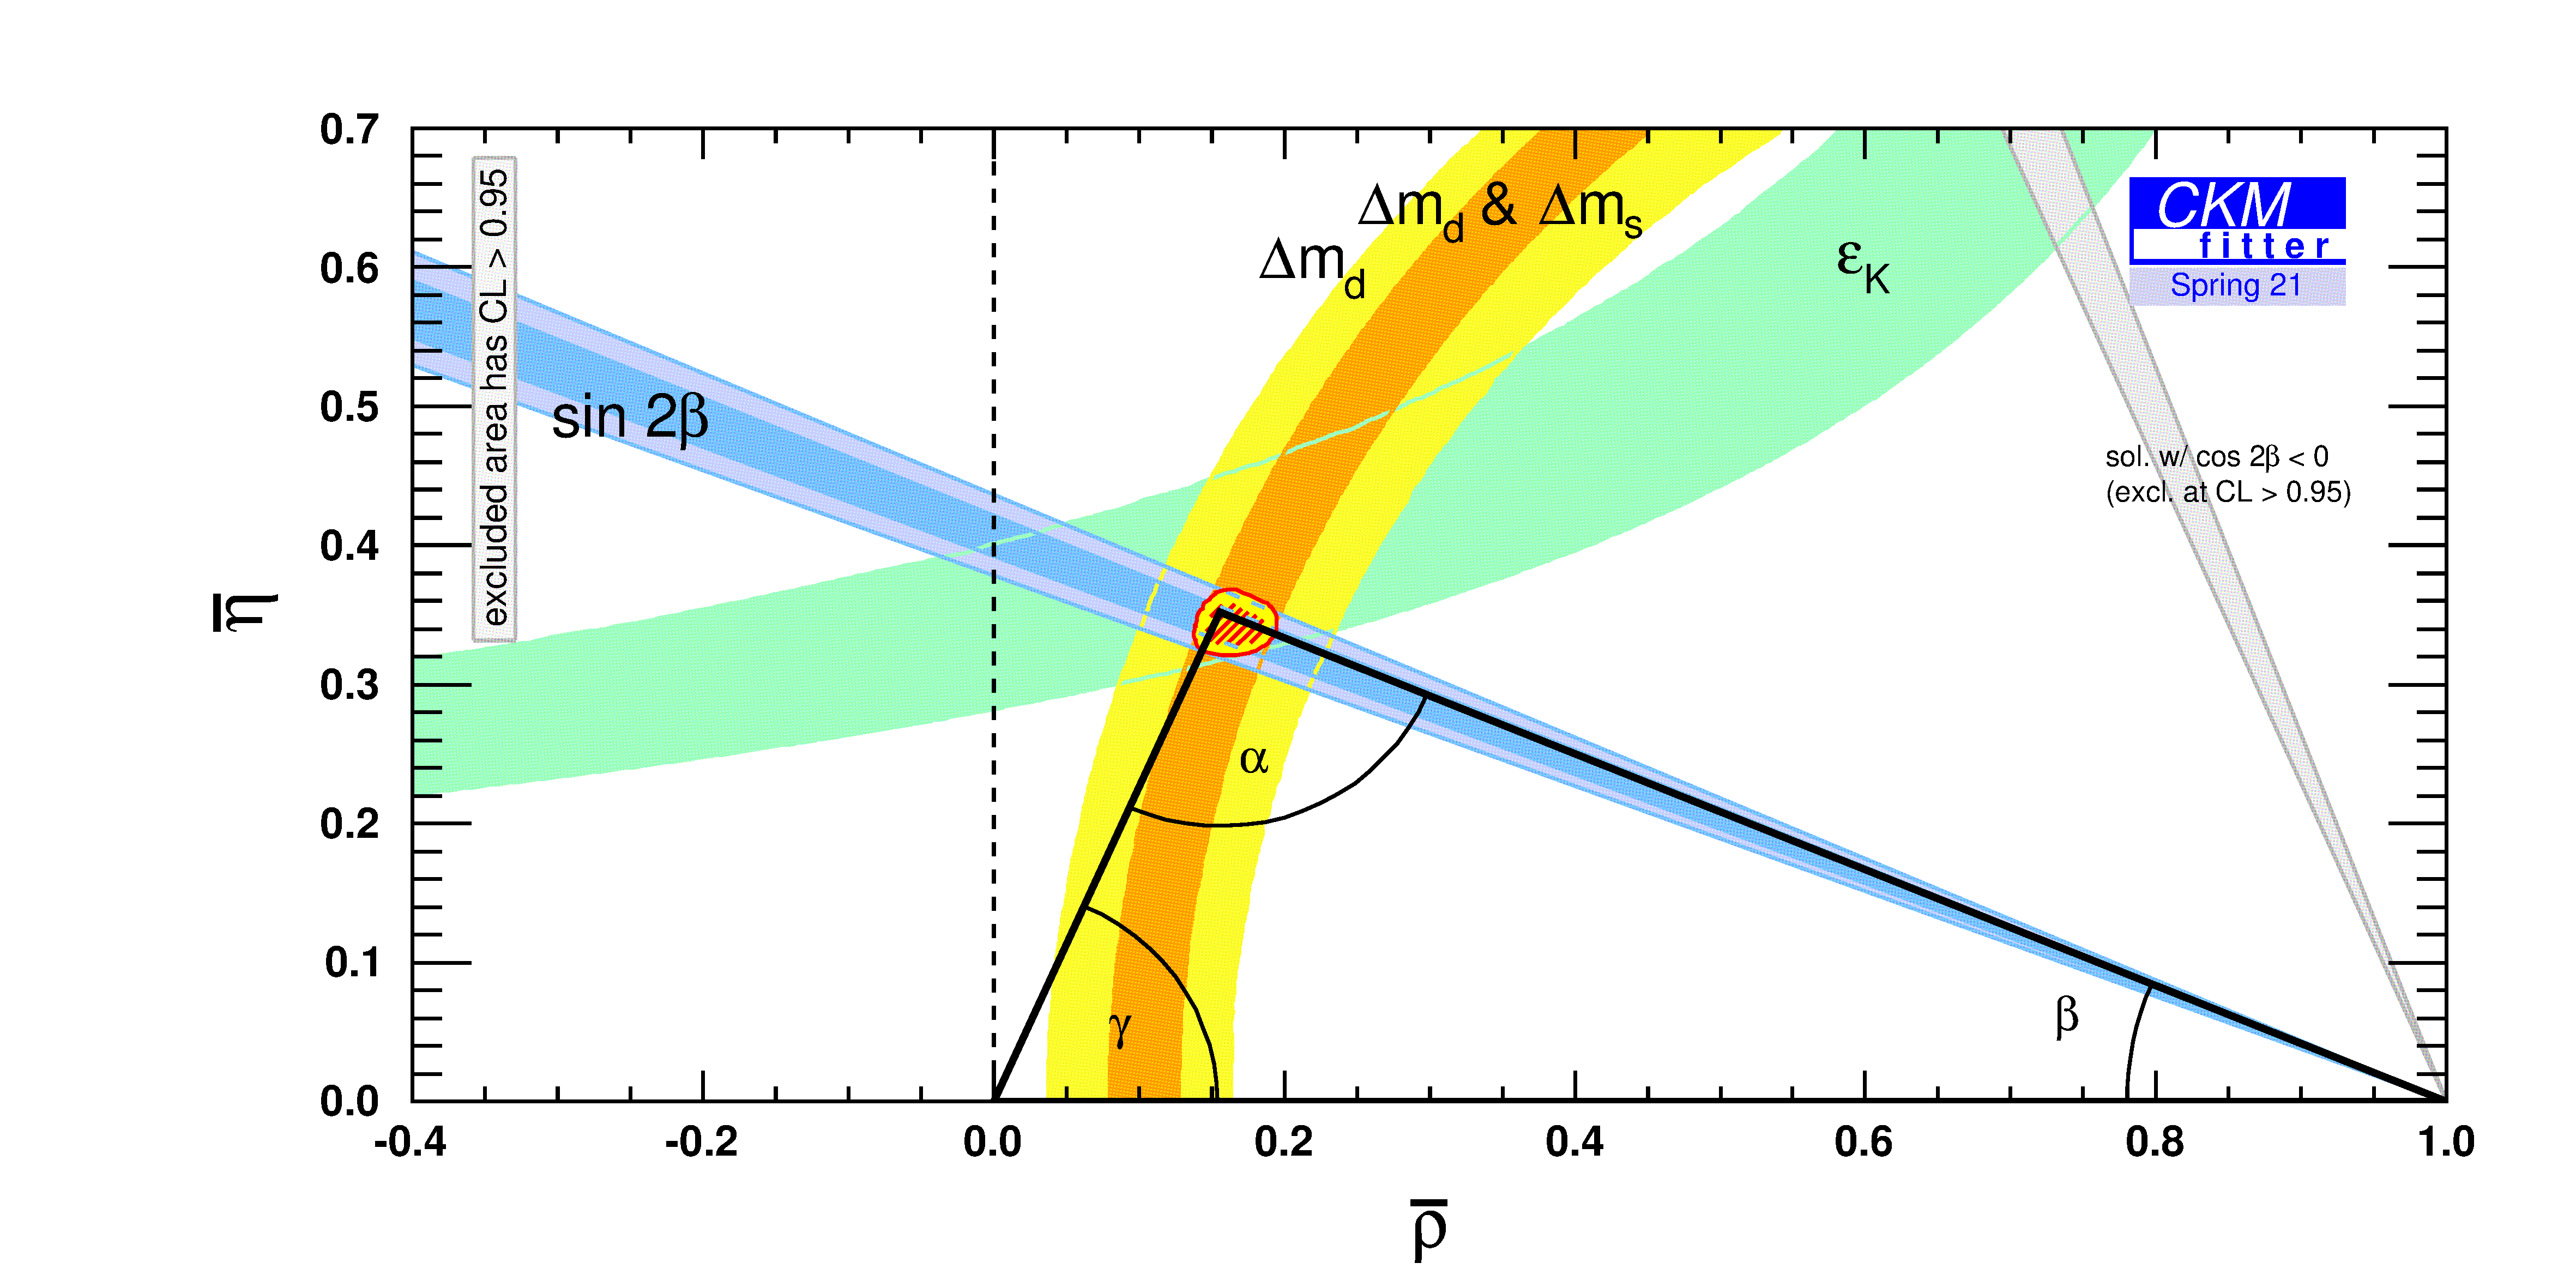
\includegraphics[width = 1.0\textwidth]{Plots/ckmfitter_loop.png}
      \caption{Loop level: $\gamma = \big(65.5^{+1.1}_{-2.7}\big)^\circ$}
    \end{subfigure}
    \vspace{-0.3cm}
    \captionsetup{justification=centering}
    \caption*{\centering\tiny CKMfitter Group (J. Charles et al.), Eur. Phys. J. C41, 1-131 (2005), updated results and plots available at: \href{http://ckmfitter.in2p3.fr}{http://ckmfitter.in2p3.fr}}
  \end{figure}
\end{frame}

\begin{frame}{Sensitivity through interference}
  \begin{center}
    \Large Measure $\gamma$ through interference effects in $B^\pm\to DK^\pm$
  \end{center}
  \begin{figure}[H]
    \centering
    \begin{subfigure}{0.5\textwidth}
      \centering
      \begin{fmffile}{fgraph/fgraph_BtoDK1}
        \setlength{\unitlength}{0.4cm}
        \begin{fmfgraph*}(6,6)
          \fmfstraight
          \fmfleft{i1,B,i2,t1,t2,t3,t9,t10}
          \fmfright{o1,D,o2,t4,t5,o3,K,o4}
          \fmflabel{$\bar{u}$}{i1}
          \fmflabel{$b$}{i2}
          \fmfv{l.d=20,l.a=180,l={$B^-$\mylbrace{30}{-8}}}{B}
          \fmflabel{$\bar{u}$}{o1}
          \fmflabel{$c$}{o2}
          \fmflabel{$\bar{u}$}{o3}
          \fmflabel{$s$}{o4}
          \fmfv{l.d=15,l.a=0,l={\myrbrace{30}{-12}}$D^0$}{D}
          \fmfv{l.d=15,l.a=0,l={\myrbrace{30}{11}}$K^-$}{K}
          \fmf{fermion}{o1,i1}
          \fmf{fermion,tension=1.5}{i2,v1}
          \fmf{fermion}{v1,o2}
          \fmf{phantom,tension=1.5}{t9,v2}
          \fmf{boson,label=$W$,label.side=left,tension=0}{v1,v2}
          \fmf{fermion}{v2,o4}
          \fmf{fermion}{o3,v2}
        \end{fmfgraph*}
      \end{fmffile}
      \vspace{0.5cm}
      \caption*{Favoured $B^-\to D^0K^-$}
    \end{subfigure}%
    \begin{subfigure}{0.5\textwidth}
      \centering
      \begin{fmffile}{fgraph/fgraph_BtoDK2}
        \setlength{\unitlength}{0.4cm}
        \begin{fmfgraph*}(6,6)
          \fmfstraight
          \fmfleft{i1,t1,t2,B,t9,t10,i2}
          \fmfright{o1,K,o2,t4,t5,o3,D,o4}
          \fmflabel{$\bar{u}$}{i1}
          \fmflabel{$b$}{i2}
          \fmfv{l.d=20,l.a=180,l={$B^-$\mylbrace{100}{-8}}}{B}
          \fmflabel{$\bar{u}$}{o1}
          \fmflabel{$s$}{o2}
          \fmflabel{$\bar{c}$}{o3}
          \fmflabel{$u$}{o4}
          \fmfv{l.d=15,l.a=0,l={\myrbrace{30}{13}}$\bar{D^0}$}{D}
          \fmfv{l.d=15,l.a=0,l={\myrbrace{30}{-13}}$K^-$}{K}
          \fmf{fermion}{o1,i1}
          \fmf{fermion,tension=1.5}{i2,v1}
          \fmf{fermion}{v1,o4}
          \fmf{phantom,tension=1.5}{t2,v2}
          \fmf{boson,label=$W$,label.side=left,tension=0}{v1,v2}
          \fmf{fermion}{v2,o2}
          \fmf{fermion}{o3,v2}
        \end{fmfgraph*}
      \end{fmffile}
      \vspace{0.5cm}
      \caption*{Suppressed $B^-\to\bar{D^0}K^-$}
    \end{subfigure}
  \end{figure}
  \vspace{-0.3cm}
  \begin{itemize}
    \item{Superposition of $D^0$ and $\bar{D^0}$}
    \begin{itemize}
      \item{Consider $D^0$/$\bar{D^0}$ decays to the same final state, such as $D\to K^+K^-$}
    \end{itemize}
    \item{$b\to u\bar{c}s$ and $b\to c\bar{u}s$ interference $\to$ Sensitivity to $\gamma$}
  \end{itemize}
  \vspace{-0.3cm}
  \begin{center}
    $\mathcal{A}(B^-)=\mathcal{A}_B\Big(\mathcal{A}_{D^0} + r_Be^{i(\delta_B - \gamma)}\mathcal{A}_{\bar{D^0}}\Big)$ \\
    $\mathcal{A}(B^+)=\mathcal{A}_B\Big(\mathcal{A}_{\bar{D^0}} + r_Be^{i(\delta_B + \gamma)}\mathcal{A}_{D^0}\Big)$ \\
  \end{center}
\end{frame}

\begin{frame}{Summary of LHCb \texorpdfstring{$\gamma$}{gamma} measurements}
  \begin{center}
    {\Large Our most precise knowledge of $\gamma$ comes from the combination of $\gamma$ and charm mixing parameters}\\~\\
    {\large LHCb-CONF-2022-003}
  \end{center}
  \begin{figure}
    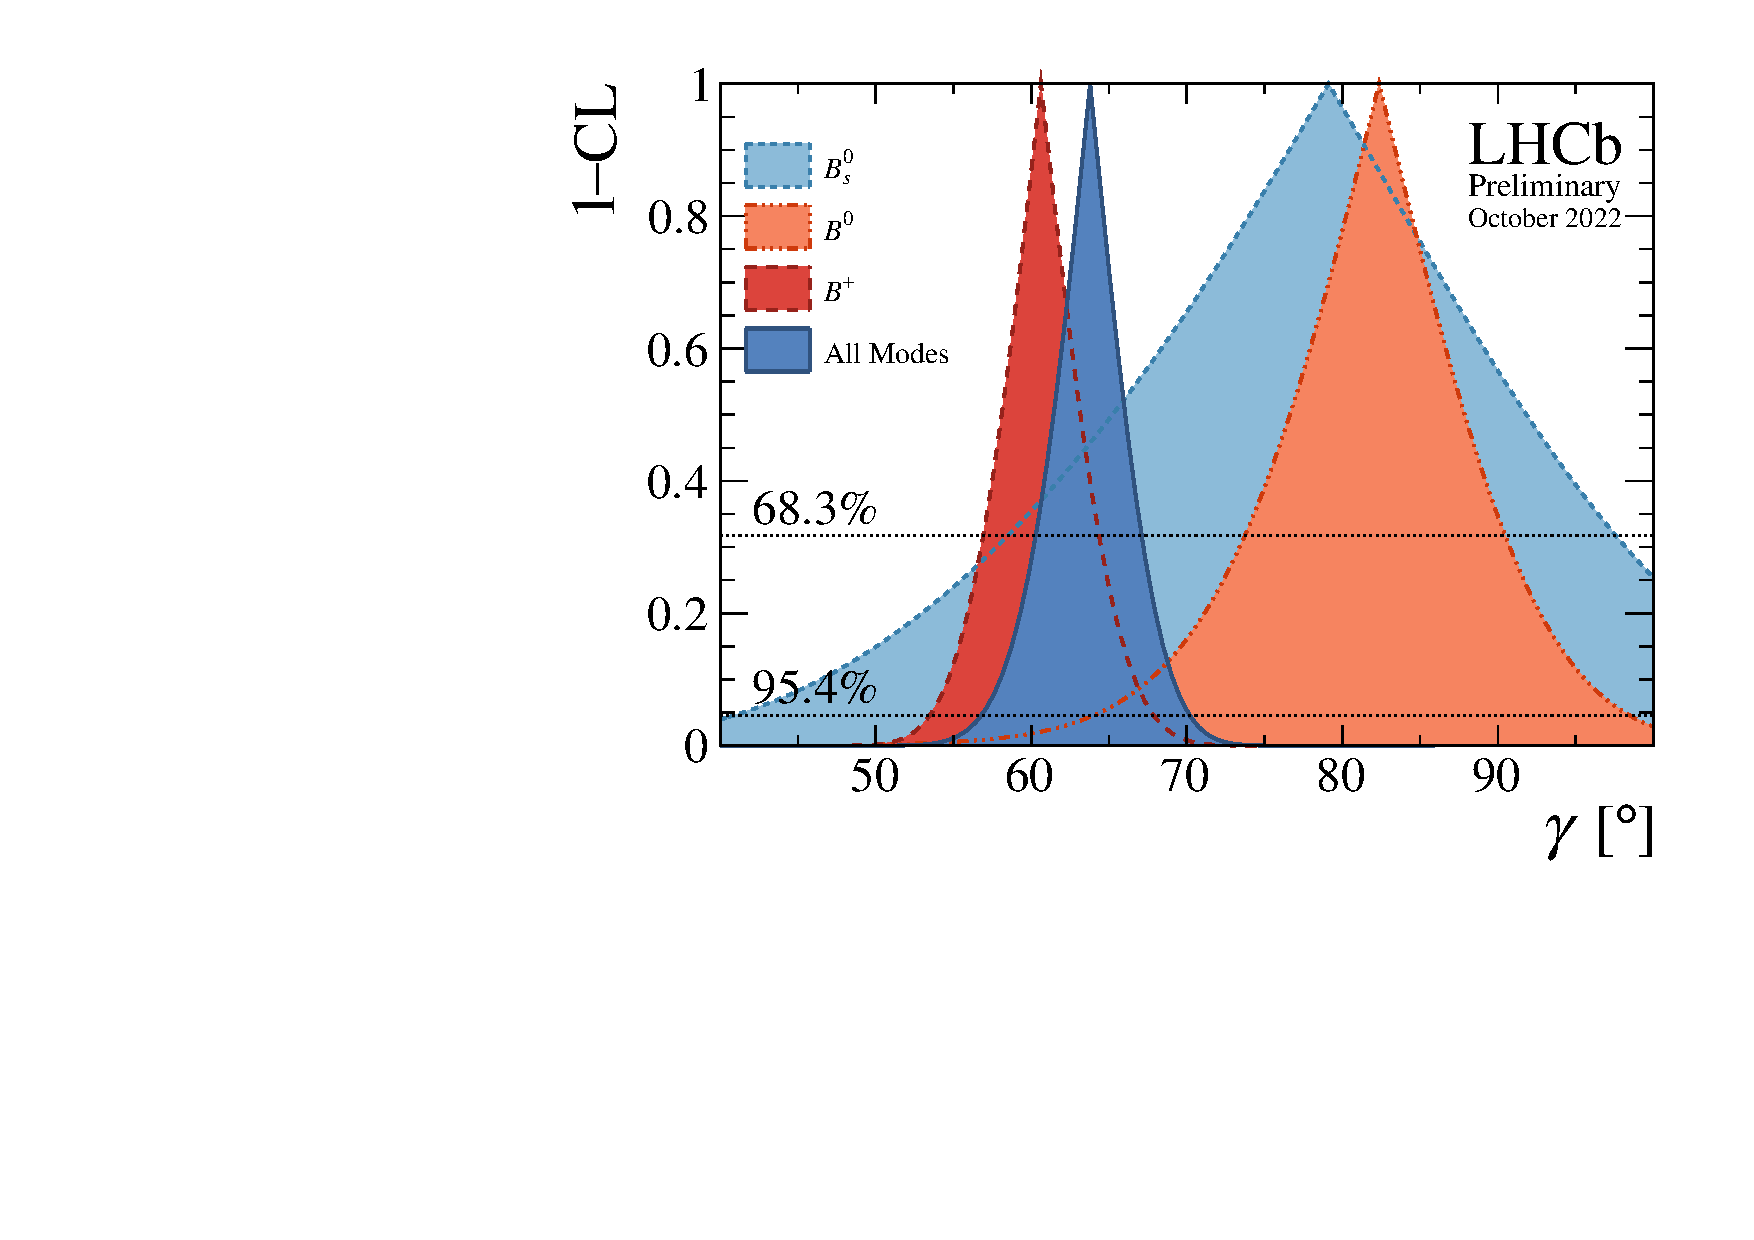
\includegraphics[height=4.0cm]{Plots/gammacharm_lhcb_comp_flavour.pdf}
    \vspace{-0.5cm}
    \caption*{\tiny\href{https://lhcbproject.web.cern.ch/Publications/LHCbProjectPublic/LHCb-CONF-2022-003.html}{LHCb-CONF-2022-003}}
  \end{figure}
  \vspace{-0.5cm}
  \begin{center}
    Most precise determination from a single experiment: $\gamma = (63.8^{+3.5}_{-3.7})^\circ$\\
    Contributions from the $B^\pm$ dominate, but all measurements are consistent
  \end{center}
\end{frame}

\begin{frame}{Summary of LHCb \texorpdfstring{$\gamma$}{gamma} measurements}
  \begin{center}
    {\Large Our most precise knowledge of $\gamma$ comes from the combination of $\gamma$ and charm mixing parameters}\\~\\
    {\large LHCb-CONF-2022-003}
  \end{center}
  \begin{figure}
    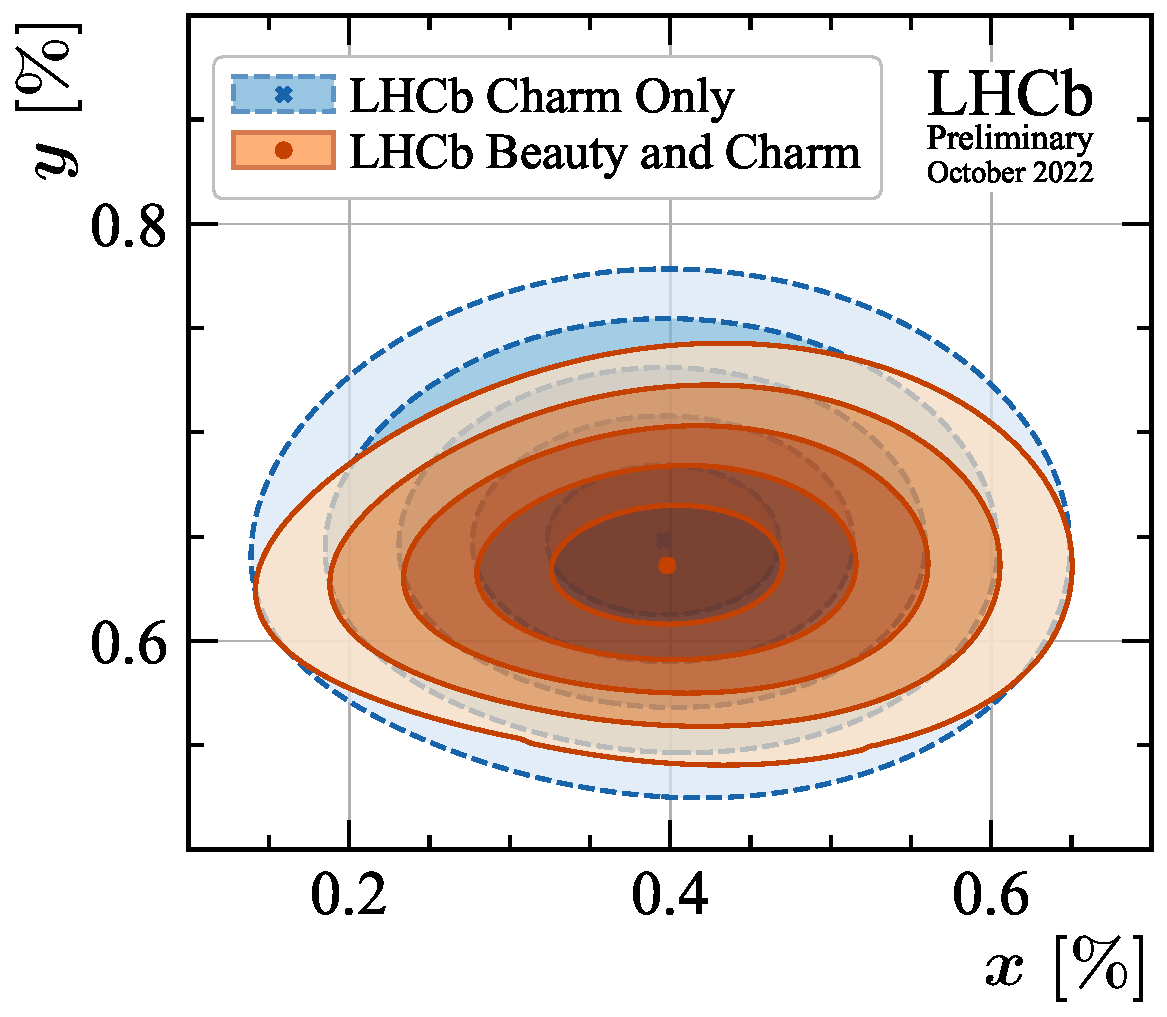
\includegraphics[height=4.0cm]{Plots/gammacharm_lhcb_xD_yD.pdf}
    \vspace{-0.5cm}
    \caption*{\tiny\href{https://lhcbproject.web.cern.ch/Publications/LHCbProjectPublic/LHCb-CONF-2022-003.html}{LHCb-CONF-2022-003}}
  \end{figure}
  \vspace{-0.5cm}
  \begin{center}
    Mixing effects to $\gamma$ measurements are approaching the statistical sensitivity\\
    The simultaneous fit improves the knowledge of $y$ significantly
  \end{center}
\end{frame}

\begin{frame}{Summary of LHCb \texorpdfstring{$\gamma$}{gamma} measurements}
  \begin{figure}
    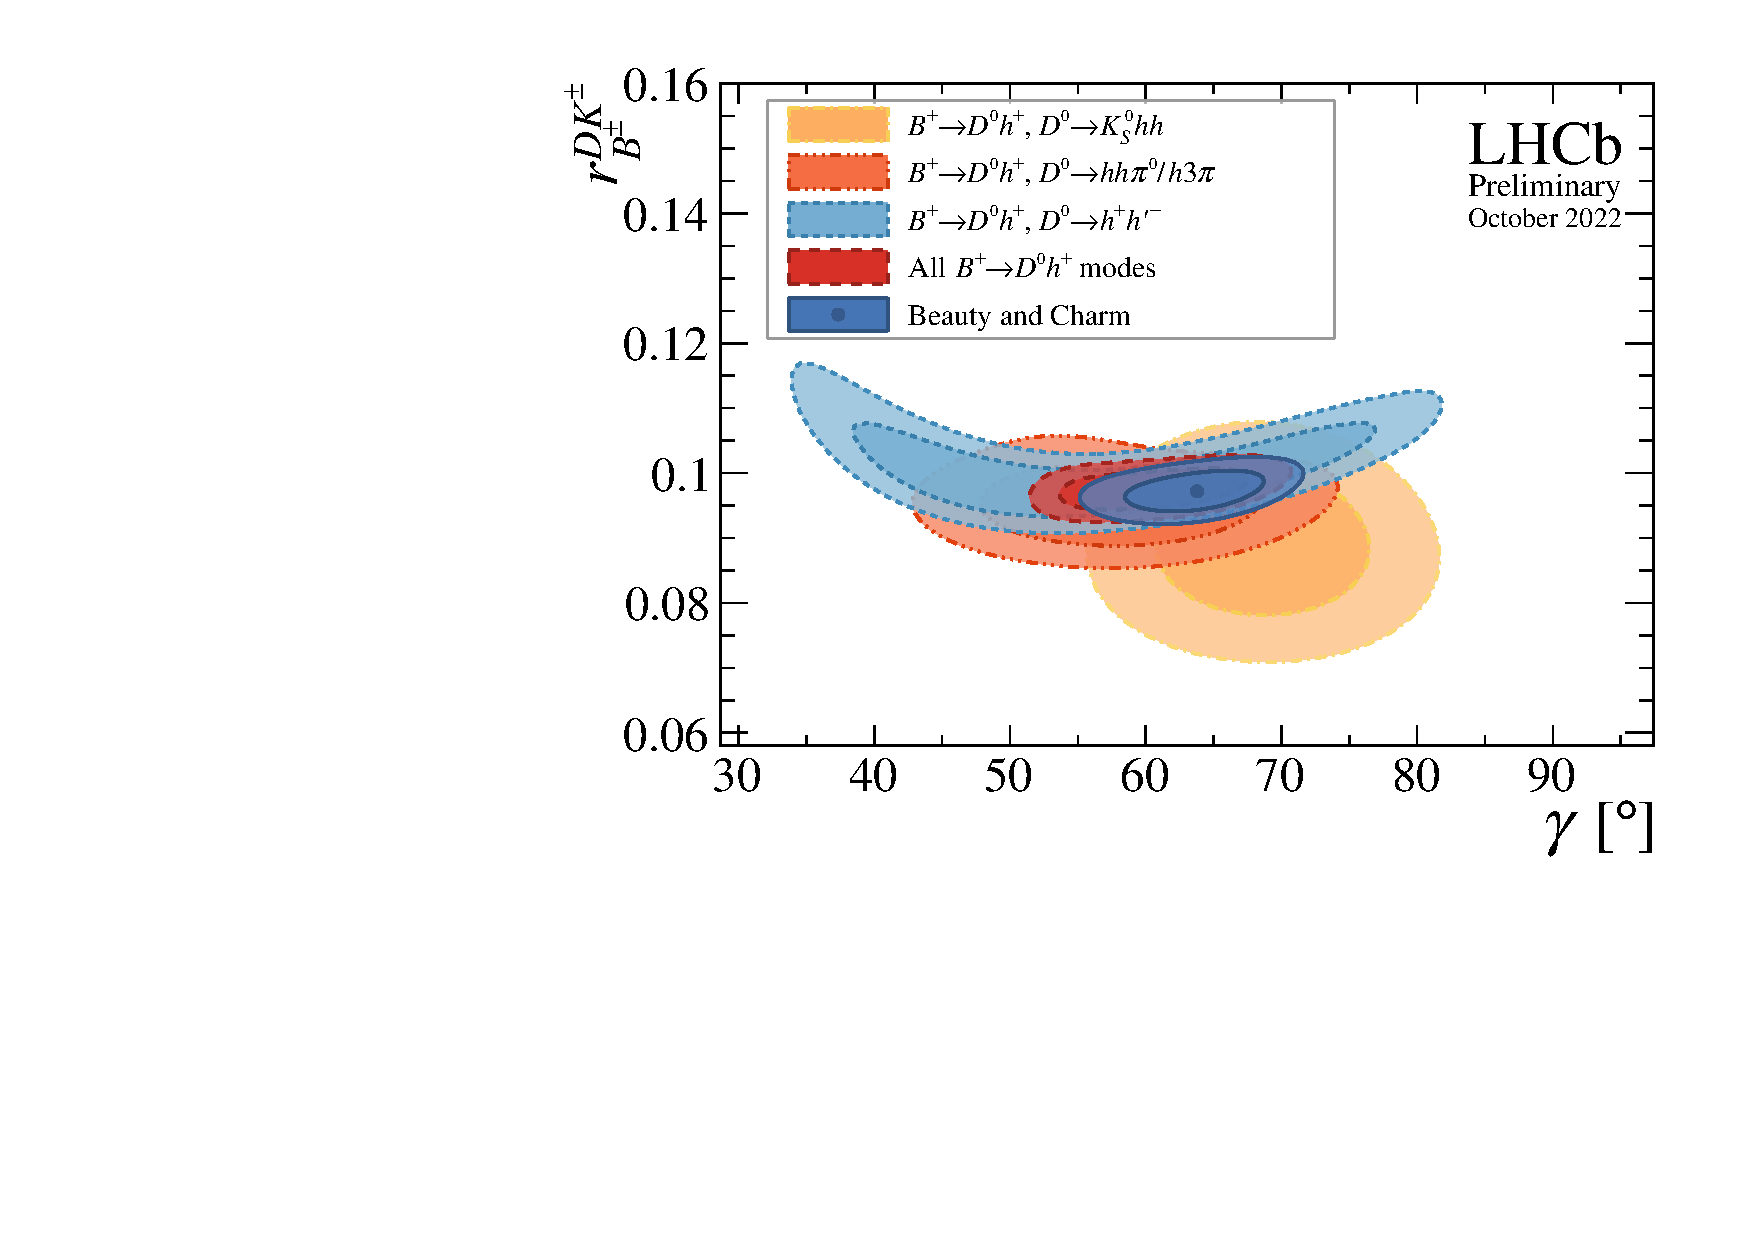
\includegraphics[height=5cm]{Plots/gammacharm_lhcb_dhch_g_r_dk.pdf}
    \vspace{-0.7cm}
    \caption*{\tiny\href{https://lhcbproject.web.cern.ch/Publications/LHCbProjectPublic/LHCb-CONF-2022-003.html}{LHCb-CONF-2022-003}}
  \end{figure}
  \vspace{-0.8cm}
  \begin{center}
    The $\gamma$ combination is mainly driven by $B^\pm\to Dh^\pm$, where:
  \end{center}
  \vspace{-0.2cm}
  \begin{columns}
    \begin{column}{0.5\textwidth}
      \begin{itemize}
        \setlength\itemsep{0.5em}
        \item{$D\to K^+K^-$, $\pi^+\pi^-$, $K^\mp\pi^\pm$}
        \item{$D\to K_S^0\pi^+\pi^-$, $K_S^0K^+K^-$}
        \item{$D\to K^\mp\pi^\pm\pi^-\pi^+$}
      \end{itemize}
    \end{column}
    \begin{column}{0.5\textwidth}
      \begin{itemize}
        \item[]{\phantom{These multi-body decays are analysed in \underline{local regions} of phase space}}
      \end{itemize}
    \end{column}
  \end{columns}
\end{frame}

\begin{frame}{Summary of LHCb \texorpdfstring{$\gamma$}{gamma} measurements}
  \begin{figure}
    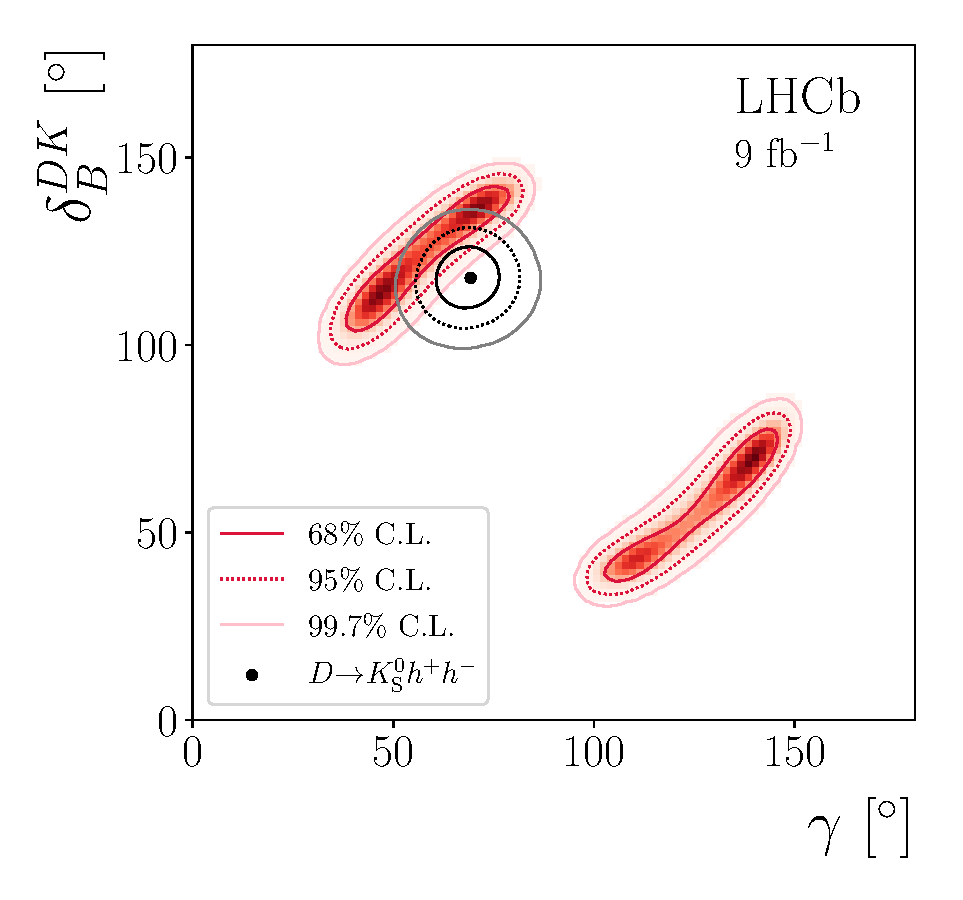
\includegraphics[height=5.1cm]{Plots/Fig6a_two_body.pdf}
    \vspace{-0.8cm}
    \caption*{\tiny\href{https://link.springer.com/article/10.1007/JHEP04(2021)081}{JHEP \textbf{04} (2021) 081}}
  \end{figure}
  \vspace{-0.8cm}
  \begin{center}
    The $\gamma$ combination is mainly driven by $B^\pm\to Dh^\pm$, where:
  \end{center}
  \vspace{-0.2cm}
  \begin{columns}
    \begin{column}{0.5\textwidth}
      \begin{itemize}
        \setlength\itemsep{0.5em}
        \item[$\rightarrow$]{$D\to K^+K^-$, $\pi^+\pi^-$, $K^\mp\pi^\pm$}
        \item[$\rightarrow$]{$D\to K_S^0\pi^+\pi^-$, $K_S^0K^+K^-$}
        \item{$D\to K^\mp\pi^\pm\pi^-\pi^+$}
      \end{itemize}
    \end{column}
    \begin{column}{0.5\textwidth}
      \begin{itemize}
        \item[]{\phantom{These multi-body decays are analysed in \underline{local regions} of phase space}}
      \end{itemize}
    \end{column}
  \end{columns}
\end{frame}

\begin{frame}{Summary of LHCb \texorpdfstring{$\gamma$}{gamma} measurements}
  \begin{figure}
    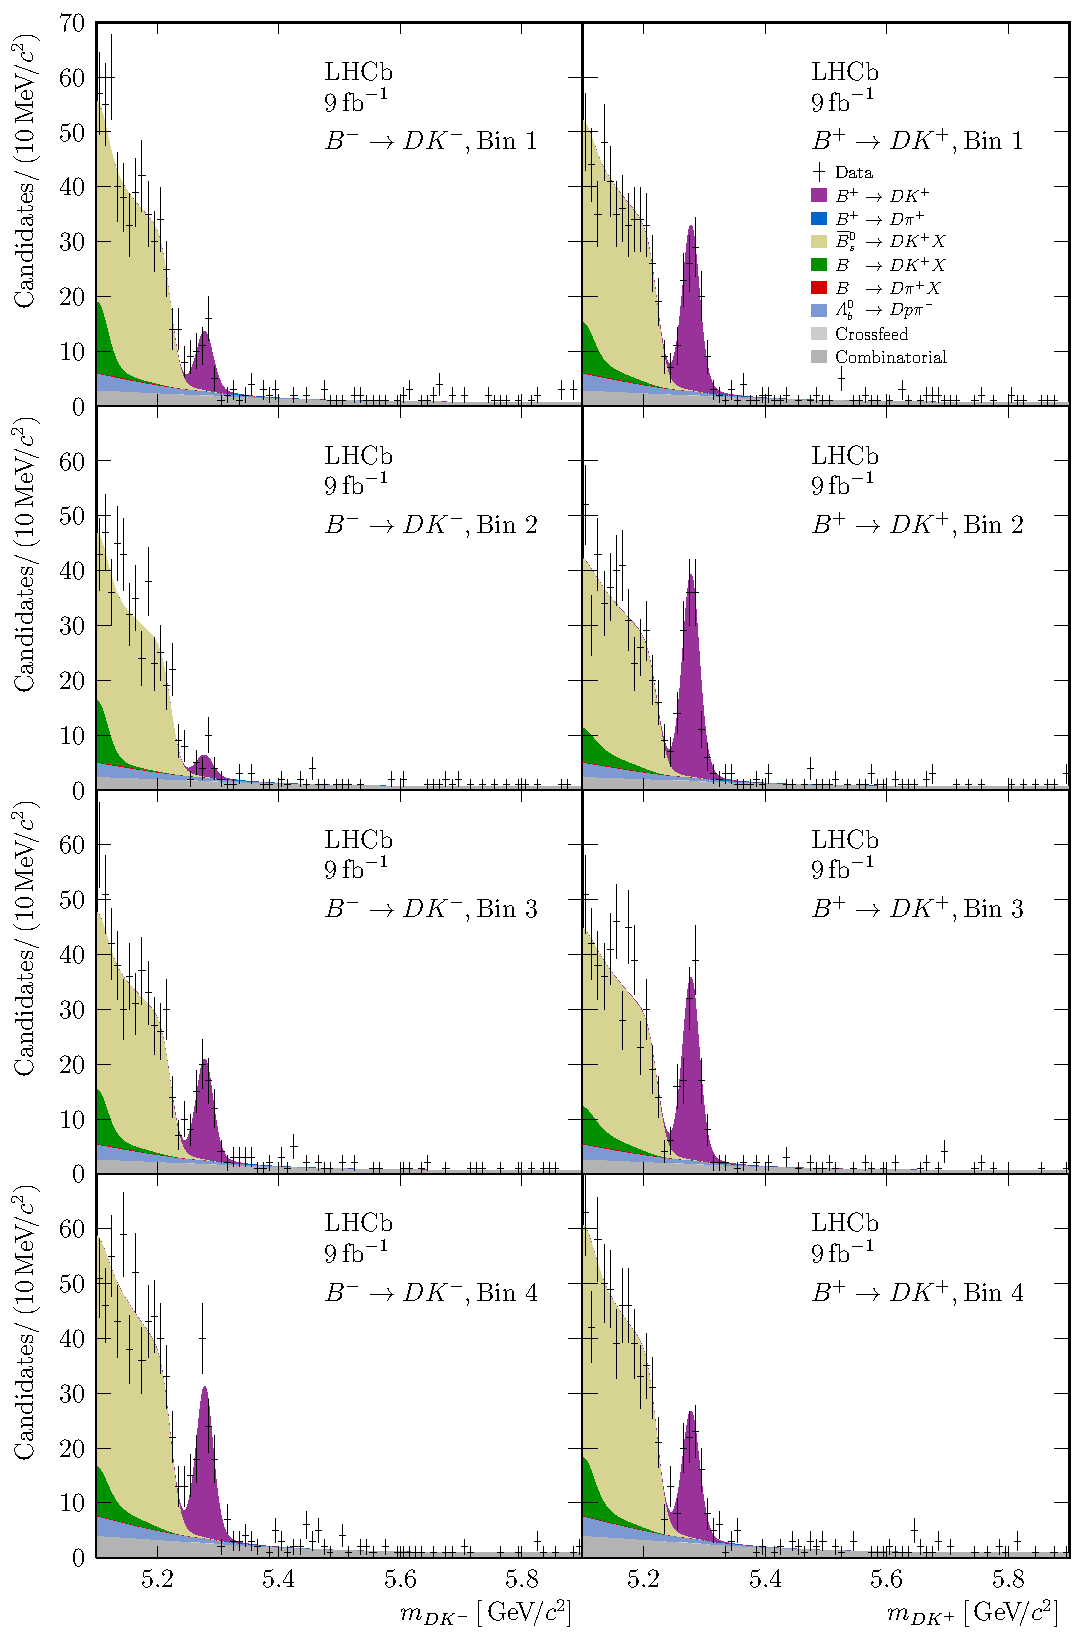
\includegraphics[height=4cm,trim={0 14.35cm 0 7.07cm},clip=true]{Plots/Fig3_K3pi.pdf}
    \vspace{0.1cm}
    \caption*{\tiny\href{https://arxiv.org/abs/2209.03692}{arXiv:2209.03692}}
  \end{figure}
  \vspace{-0.6cm}
  \begin{center}
    The $\gamma$ combination is mainly driven by $B^\pm\to Dh^\pm$, where:
  \end{center}
  \vspace{-0.2cm}
  \begin{columns}
    \begin{column}{0.5\textwidth}
      \begin{itemize}
        \setlength\itemsep{0.5em}
        \item{$D\to K^+K^-$, $\pi^+\pi^-$, $K^\mp\pi^\pm$}
        \item{$D\to K_S^0\pi^+\pi^-$, $K_S^0K^+K^-$}
        \item[$\rightarrow$]{$D\to K^\mp\pi^\pm\pi^-\pi^+$}
      \end{itemize}
    \end{column}
    \begin{column}{0.5\textwidth}
      \begin{itemize}
        \item[]{\phantom{These multi-body decays are analysed in \underline{local regions} of phase space}}
      \end{itemize}
    \end{column}
  \end{columns}
\end{frame}

\begin{frame}{Summary of LHCb \texorpdfstring{$\gamma$}{gamma} measurements}
  \begin{figure}
    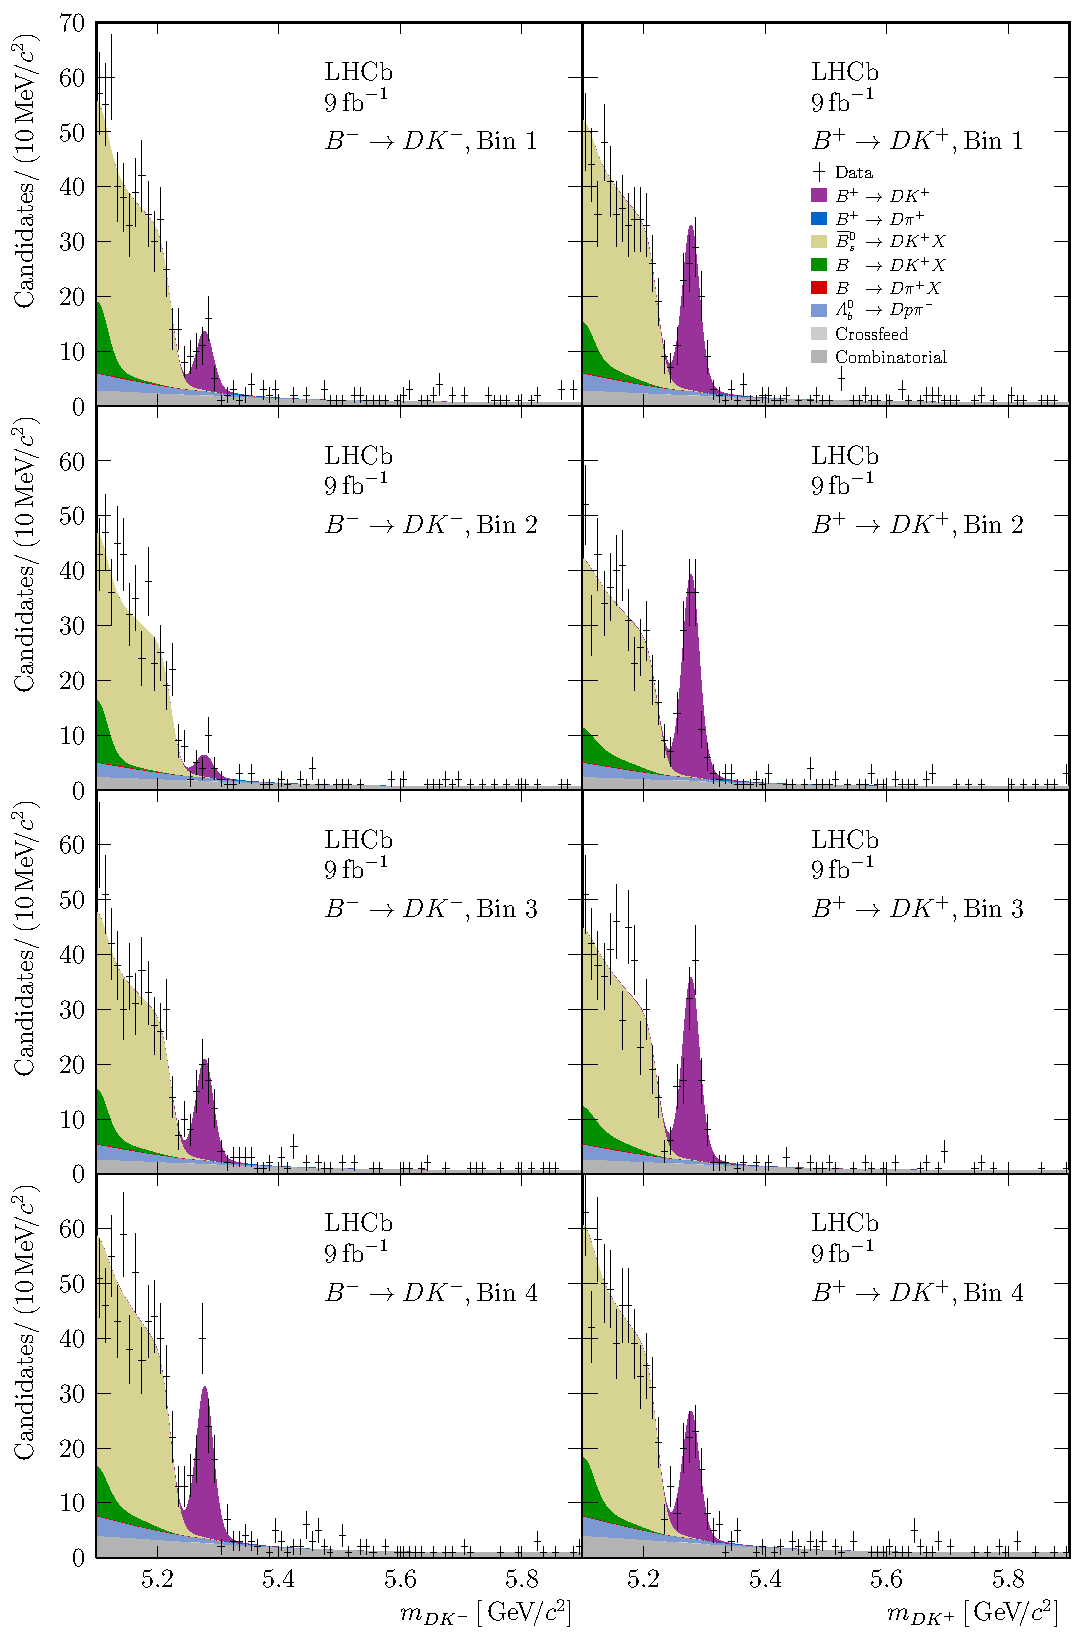
\includegraphics[height=4cm,trim={0 14.35cm 0 7.07cm},clip=true]{Plots/Fig3_K3pi.pdf}
    \vspace{0.1cm}
    \caption*{\tiny\href{https://arxiv.org/abs/2209.03692}{arXiv:2209.03692}}
  \end{figure}
  \vspace{-0.6cm}
  \begin{center}
    The $\gamma$ combination is mainly driven by $B^\pm\to Dh^\pm$, where:
  \end{center}
  \vspace{-0.2cm}
  \begin{columns}
    \begin{column}{0.5\textwidth}
      \begin{itemize}
        \setlength\itemsep{0.5em}
        \item{$D\to K^+K^-$, $\pi^+\pi^-$, $K^\mp\pi^\pm$}
        \item{$D\to K_S^0\pi^+\pi^-$, $K_S^0K^+K^-$\tikzmark{t1}}
        \item{$D\to K^\mp\pi^\pm\pi^-\pi^+$\tikzmark{t2}}
      \end{itemize}
    \end{column}
    \begin{column}{0.5\textwidth}
      \begin{itemize}
        \item[]{\tikzmark{n1}\cbox{These multi-body decays are analysed in \underline{local regions} of phase space}}
      \end{itemize}
    \end{column}
  \end{columns}
  \begin{tikzpicture}[remember picture,overlay]
    \path[draw=blue,thick,->] ([xshift=-1mm]n1) -- ([yshift=1mm]t1);
    \path[draw=blue,thick,->] ([xshift=-1mm]n1) -- ([yshift=1mm]t2);
  \end{tikzpicture}
\end{frame}

\begin{frame}[fragile]{Multi-body $D$ decays}
  \begin{center}
    This talk: Focus on multi-body $D$ decays, where interference effects vary across phase space
  \end{center}
  \vspace{-0.3cm}
  \begin{itemize}
    \setlength\itemsep{0.5em}
    \item{Strong-phase difference $\delta_D$ is a function of phase space}
    \item{Compare yields of $B^+$ and $B^-$ and determine the asymmetry \underline{in local phase space regions}}
  \end{itemize}
  \begin{equation*}
    \begin{tikzcd}[column sep=huge]
      & D^0K^- \arrow[dr, bend left = 25, "\mathcal{A}_{D^0}(\Phi)"] & \\
      B^- \arrow[ur, bend left, "\mathcal{A}_B"] \arrow[dr, bend right, "\mathcal{A}_B r_B e^{i(\delta_B - \gamma)}"'] & [5cm] & DK^- \\
      & \bar{D^0}K^- \arrow[ur, bend right = 25, "\mathcal{A}_{\bar{D^0}}(\Phi)"'] & \\
    \end{tikzcd}
  \end{equation*}
  \vspace{-0.9cm}
  \begin{align*}
    \lvert\mathcal{A}(B^-)\lvert^2&\propto\lvert\mathcal{A}_{D^0}(\Phi)\lvert^2 + r_B^2\lvert\mathcal{A}_{\bar{D^0}}(\Phi)\lvert^2 \\
    &+ 2r_B\lvert\mathcal{A}_{D^0}(\Phi)\lvert\lvert\mathcal{A}_{\bar{D^0}}(\Phi)\lvert\cos(\delta_B - \gamma + \delta_D)
  \end{align*}
\end{frame}

\begin{frame}{Multi-body $D$ decays}
  \begin{itemize}
    \setlength\itemsep{0.5em}
    \item{Interpretation of $\gamma$ from the multi-body charm decays require external inputs of the charm strong-phase differences}
    \item{The three-body decays $D\to K_S^0h^+h^-$ have been studied extensively, using an optimised phase-space binning:}
    \begin{itemize}
      \item{CLEO \href{https://doi.org/10.1103/PhysRevD.82.112006}{Phys. Rev. \textbf{D82} (2010) 112006}}
      \item{BESIII \href{https://journals.aps.org/prd/abstract/10.1103/PhysRevD.101.112002}{Phys. Rev. \textbf{D101} (2020) 112002}}
    \end{itemize}
    \item{With charm inputs from CLEO and BESIII, the measurement of $\gamma$ becomes \underline{model independent}}
  \end{itemize}
  \begin{figure}
    \centering
    \begin{subfigure}{0.5\textwidth}
      \centering
      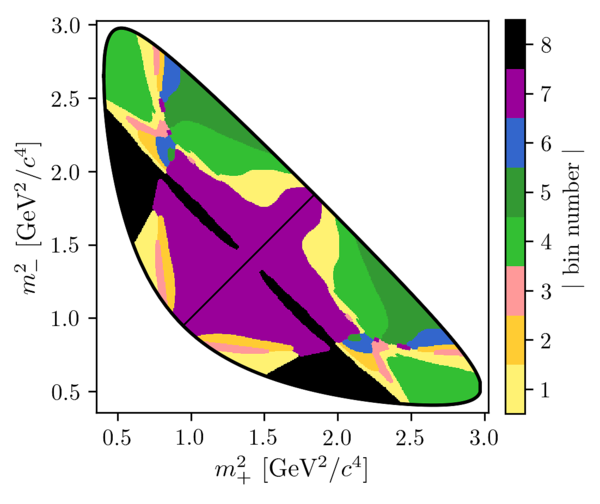
\includegraphics[height = 3.5cm]{Plots/KsPiPi_optimal.png}
      \vspace{-0.3cm}
      \caption*{$K_S^0\pi^+\pi^-$}
    \end{subfigure}%
    \begin{subfigure}{0.5\textwidth}
      \centering
      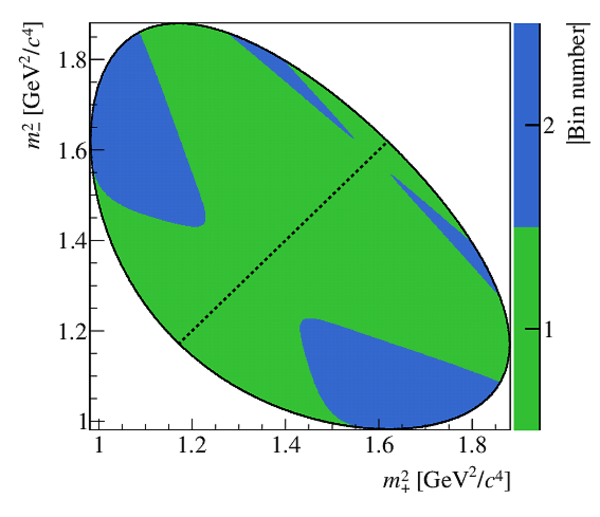
\includegraphics[height = 3.5cm]{Plots/KsKK_binning.png}
      \vspace{-0.3cm}
      \caption*{$K_S^0K^+K^-$}
    \end{subfigure}
    \vspace{-0.9cm}
    \caption*{\tiny\href{https://link.springer.com/article/10.1007/JHEP02(2021)169}{JHEP \textbf{02} (2021) 0169}}
  \end{figure}
\end{frame}

\section{Phase-space binned analysis of \texorpdfstring{$B^\pm\to[K^+K^-\pi^+\pi^-]_DK^\pm$}{B2DKD2KKpipi}}
\begin{frame}{Phase-space binned $B^\pm\to[K^+K^-\pi^+\pi^-]_DK^\pm$}
  \begin{center}
    {\Large Can also consider more complicated multi-body decays: $B^\pm\to[K^+K^-\pi^+\pi^-]_DK^\pm$}\\~\\
  \end{center}
  \vspace{-0.5cm}
  \begin{itemize}
    \setlength\itemsep{0.0em}
    \item{Phase space is 5-dimensional...}
    \item{...use an amplitude model to determine an efficient binning scheme!}
  \end{itemize}
  \vspace{-0.2cm}
  \begin{figure}
    \centering
    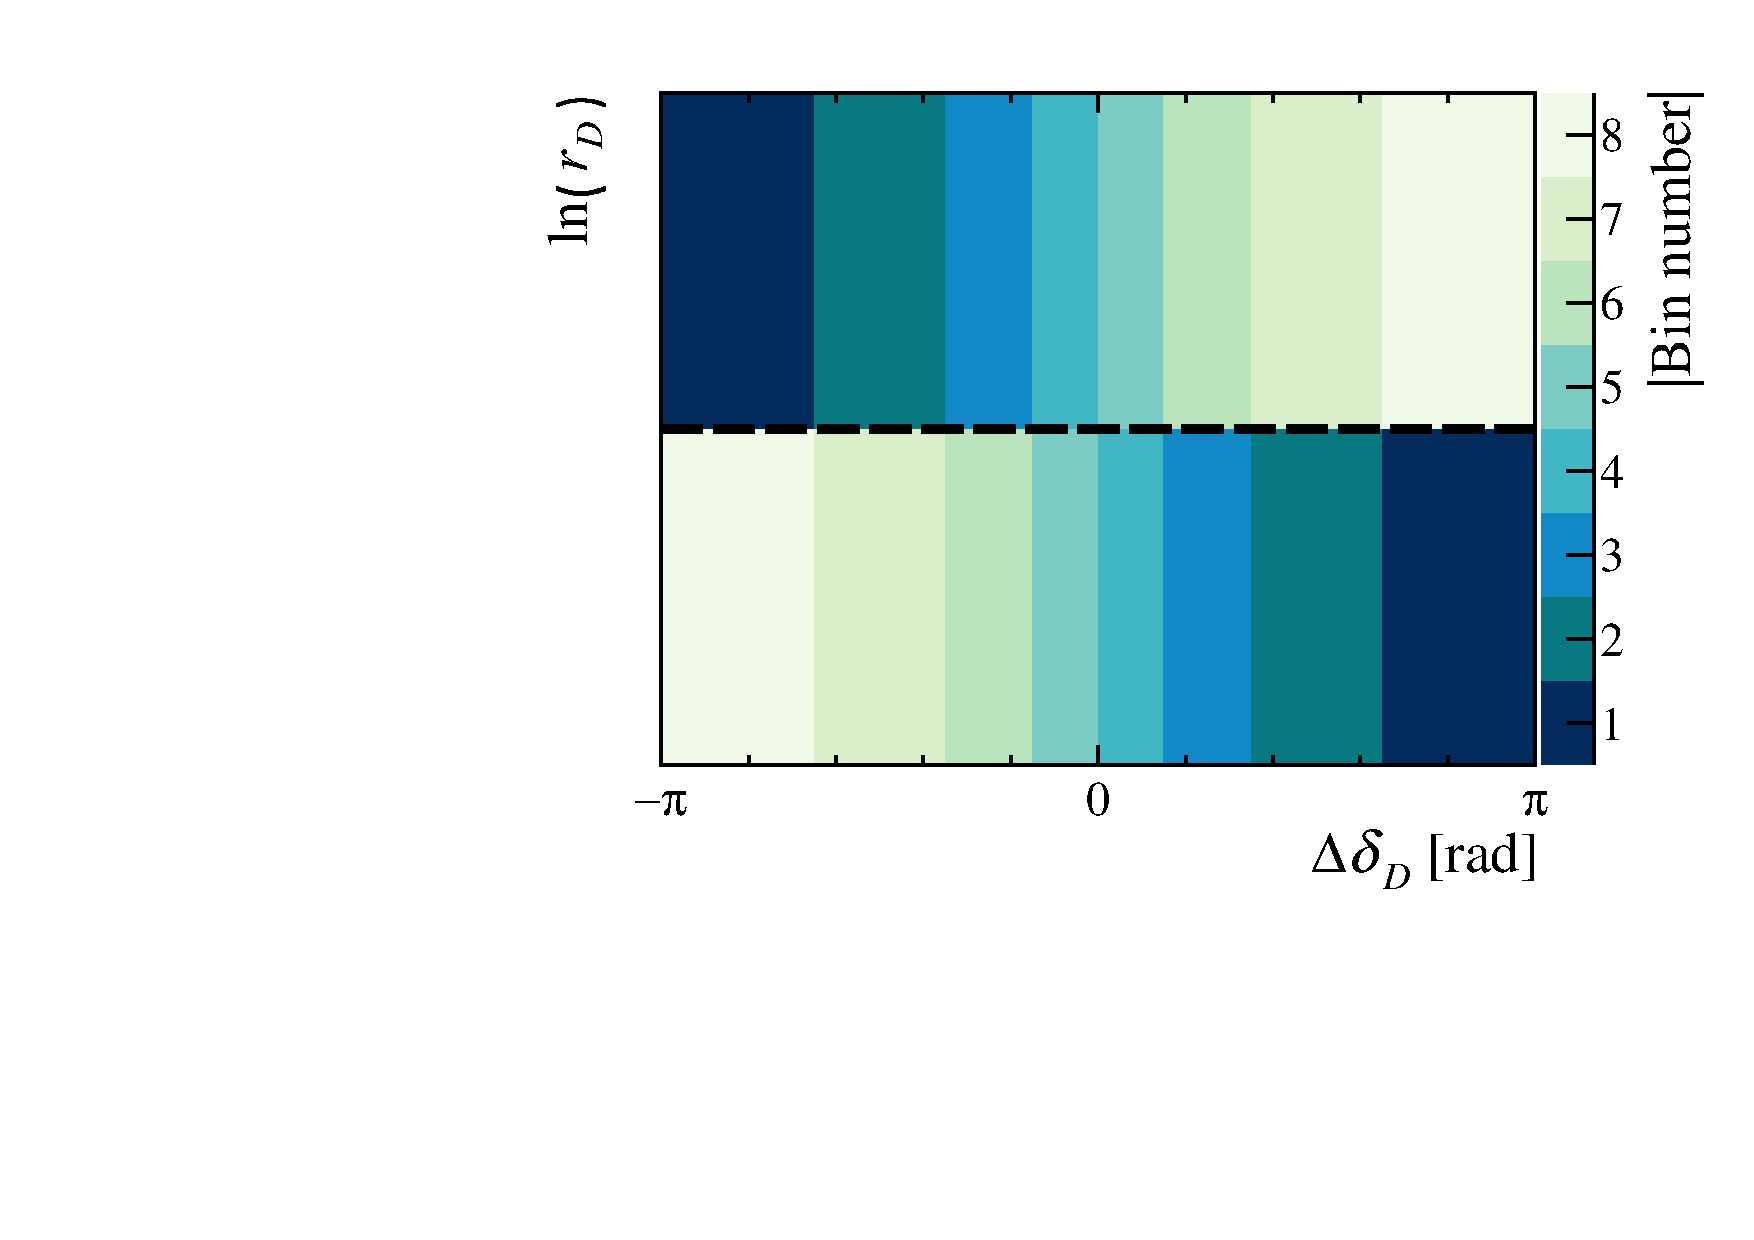
\includegraphics[width = 0.5\textwidth]{Plots/BinningSchemePlot_8Bins.pdf}
  \end{figure}
  \vspace{-0.5cm}
  \begin{center}
    Bins $i < 0$ on top, $i > 0$ below\\
    \href{https://link.springer.com/article/10.1140/epjc/s10052-023-11560-5}{Eur. Phys. J. C \textbf{83}, 547 (2023)}
  \end{center}
\end{frame}

\begin{frame}{Phase-space binned $B^\pm\to[K^+K^-\pi^+\pi^-]_DK^\pm$}
  \begin{center}
    {\large Fully charged final state $\implies$ Highly suitable for LHCb}
  \end{center}
  \begin{figure}
    \centering
    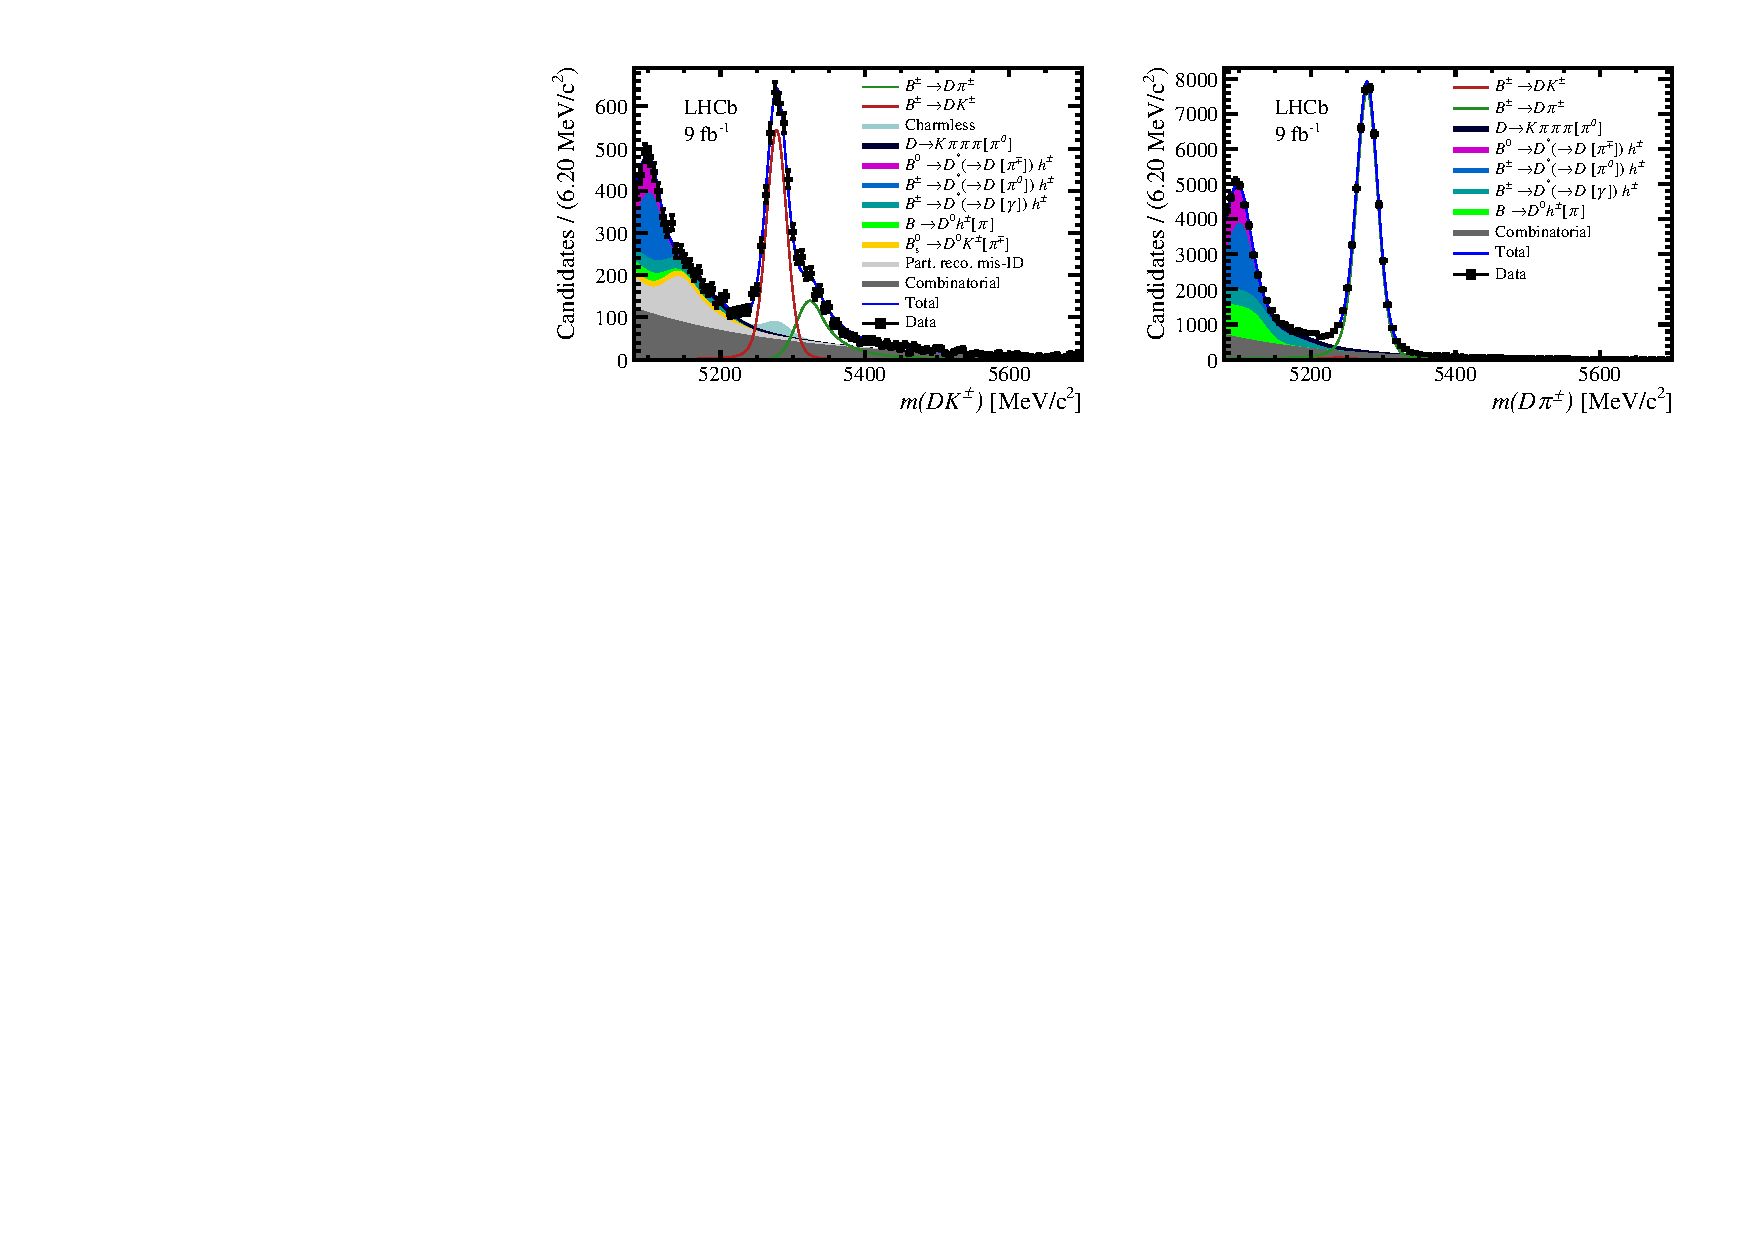
\includegraphics[width = 1.0\textwidth,trim={0 0 0 0},clip=true]{Plots/d2kkpipi_fiveL_allDP.pdf}
    \caption*{\tiny\href{https://link.springer.com/article/10.1140/epjc/s10052-023-11560-5}{Eur. Phys. J. C \textbf{83}, 547 (2023)}}
  \end{figure}
  \vspace{-0.5cm}
  \begin{itemize}
    \item{$B^\pm\to[K^+K^-\pi^+\pi^-]_Dh^\pm$ signal yield:}
    \begin{itemize}
      \item{$B^\pm\to DK^\pm$: $3026 \pm 38$}
      \item{$B^\pm\to D\pi^\pm$: $44349 \pm 218$}
    \end{itemize}
  \end{itemize}
\end{frame}

\begin{frame}{Phase-space binned $B^\pm\to[K^+K^-\pi^+\pi^-]_DK^\pm$}
  \begin{figure}
    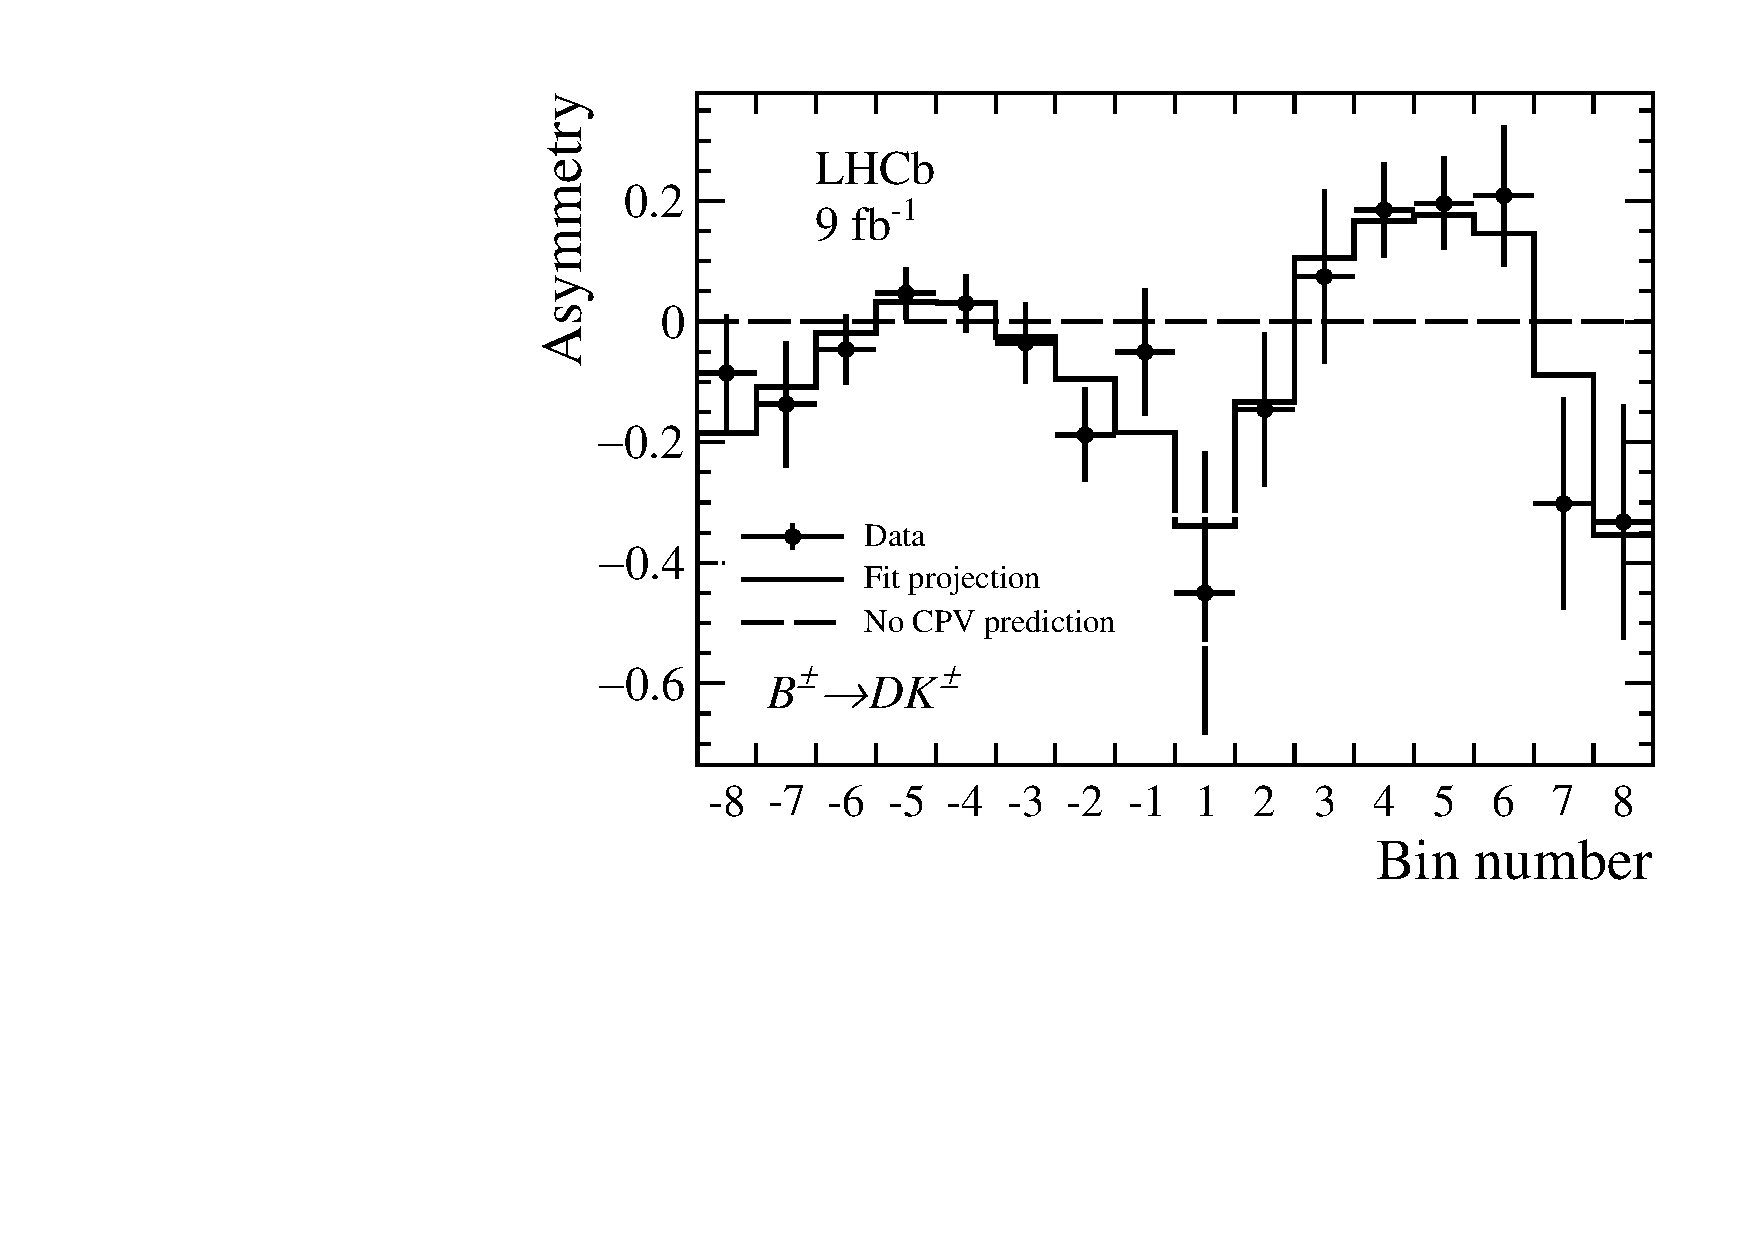
\includegraphics[height = 5cm]{Plots/BinAsymmetries_dk.pdf}
    \vspace{-0.4cm}
    \caption*{\tiny\href{https://link.springer.com/article/10.1140/epjc/s10052-023-11560-5}{Eur. Phys. J. C \textbf{83}, 547 (2023)}}
  \end{figure}
  \vspace{-0.5cm}
  \begin{itemize}
    \setlength\itemsep{0.5em}
    \item{Clear bin asymmetries are seen, and the non-trivial distribution is driven by the change in strong-phase differences across phase space}
    \item{While the interpretation of $\gamma$ require charm inputs, the observed bin asymmetries are model independent}
  \end{itemize}
\end{frame}

\begin{frame}{Phase-space integrated $B^\pm\to[K^+K^-\pi^+\pi^-]_DK^\pm$}
  \begin{center}
    {\large Additionally, one can measure the phase-space integrated asymmetries and measure additional $C\!P$-violating observables}
  \end{center}
  \begin{figure}
    \centering
    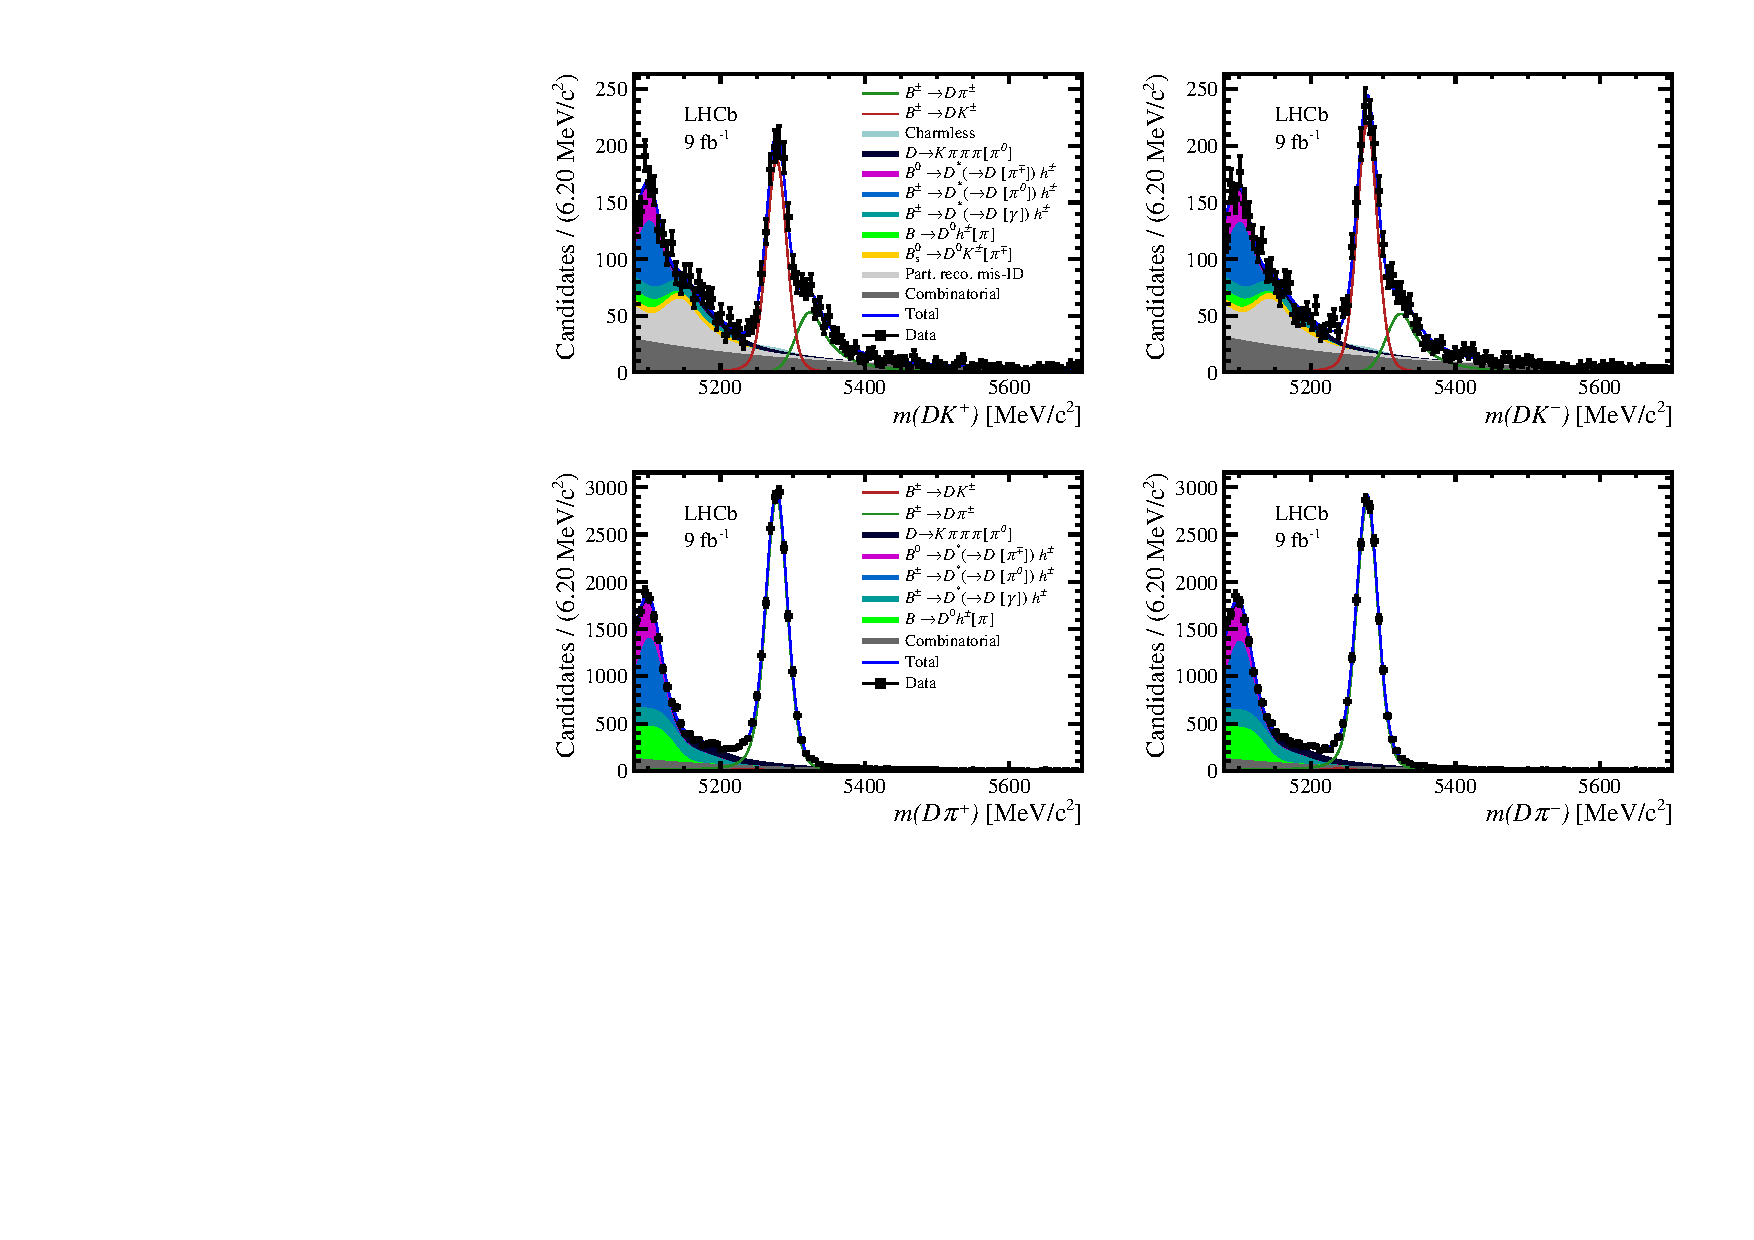
\includegraphics[width = 1.0\textwidth,trim={0 7cm 0 0},clip=true]{Plots/d2kkpipi_fiveL_allDP_GLW.pdf}
    \vspace{-0.6cm}
    \caption*{\tiny\href{https://link.springer.com/article/10.1140/epjc/s10052-023-11560-5}{Eur. Phys. J. C \textbf{83}, 547 (2023)}}
  \end{figure}
  \vspace{-0.4cm}
  \begin{center}
    {\large More $B^-$ candidates because $D^0\to K^+K^-\pi^+\pi^-$ is predominantly \underline{$C\!P$-even} (\href{https://journals.aps.org/prd/abstract/10.1103/PhysRevD.107.032009}{Phys. Rev. D \textbf{107} 032009})}
  \end{center}
\end{frame}

\begin{frame}{Phase-space binned $B^\pm\to[K^+K^-\pi^+\pi^-]_DK^\pm$}
  \begin{center}
    \large From the phase-space binned asymmetries, we obtain:
  \end{center}
  \begin{itemize}
    \item{$\gamma = (116^{+12}_{-14})^\circ$}
    \item{$\delta_D^{DK} = (81^{+12}_{-14})^\circ$}
    \item{$r_B^{DK} = 0.110^{+0.020}_{-0.020}$}
  \end{itemize}
  \vspace{-0.2cm}
  \begin{figure}[htb]
    \centering
    \begin{subfigure}{0.5\textwidth}
      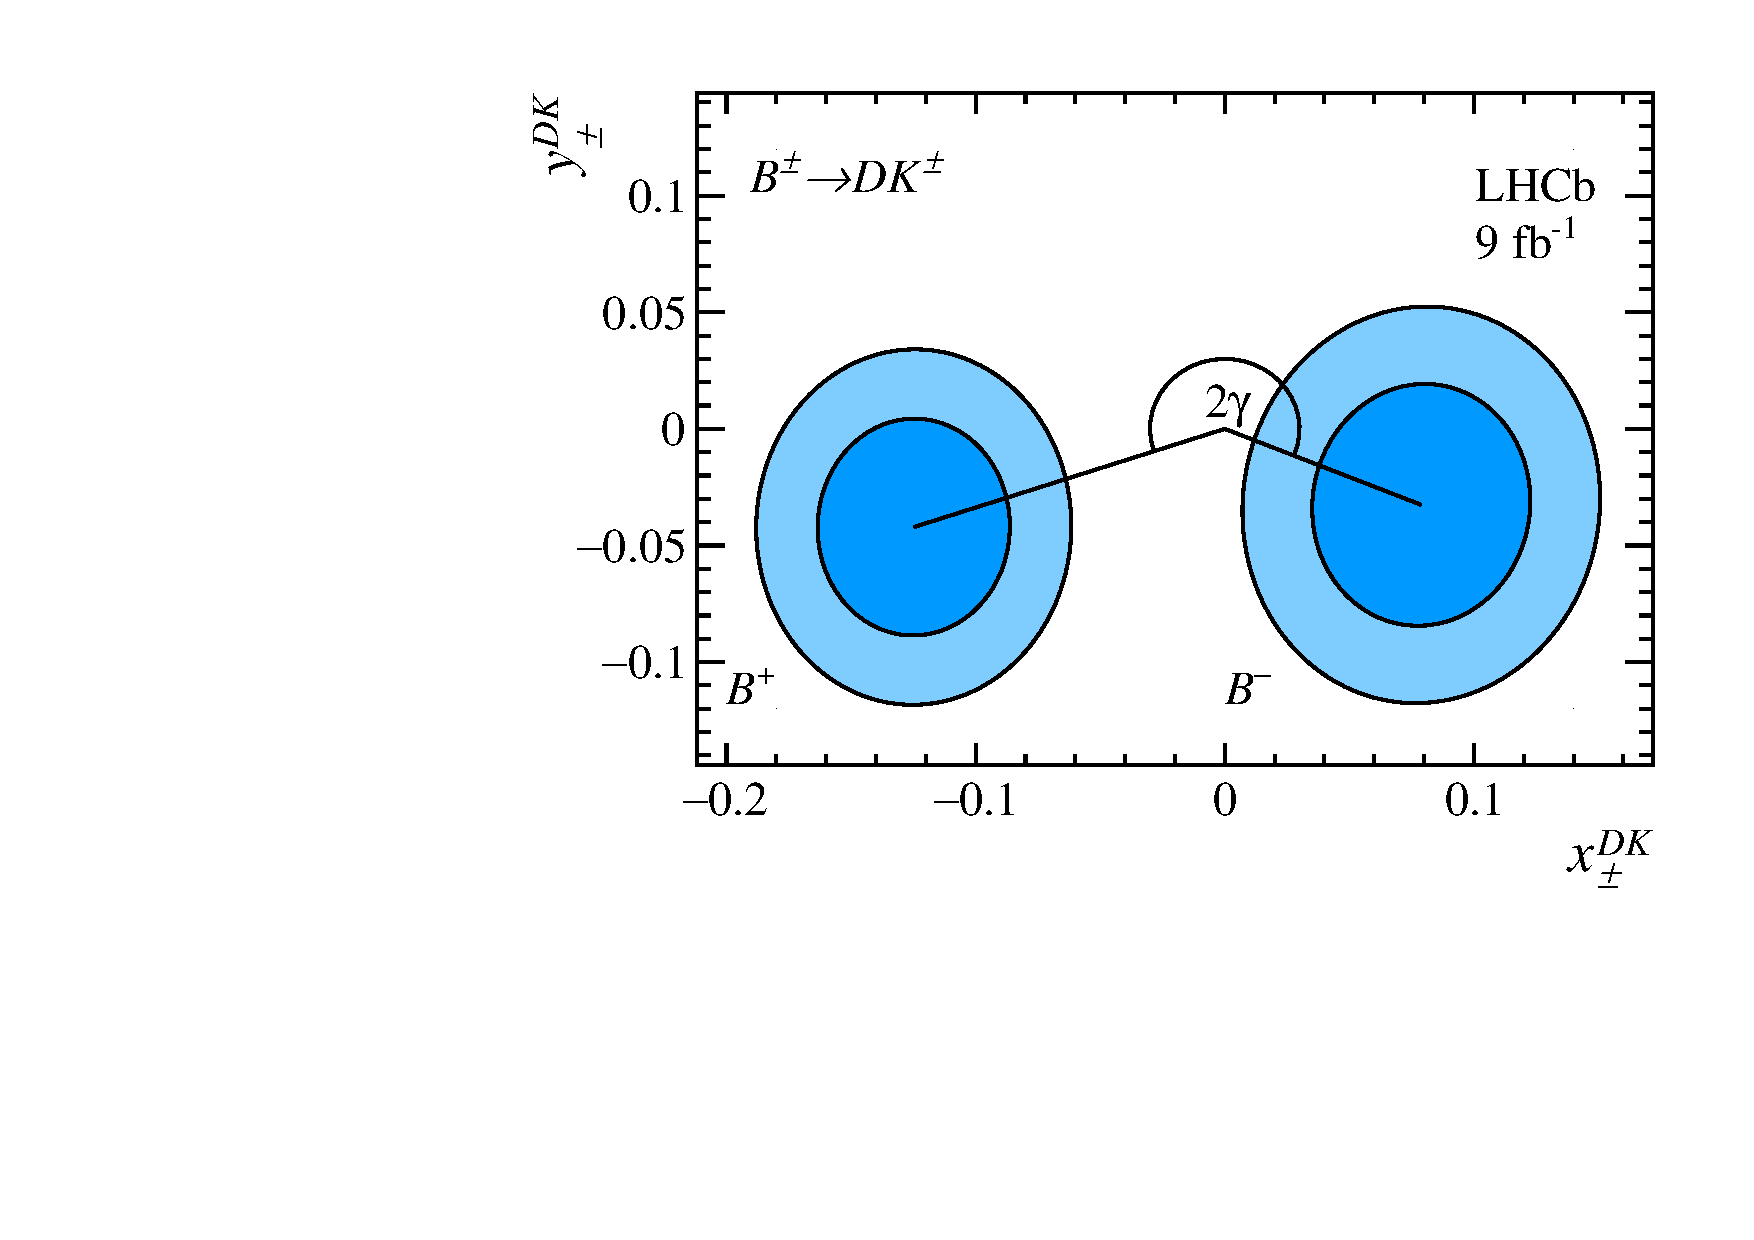
\includegraphics[width=1\textwidth]{Plots/B2DK_CP_Observables_Contours.pdf}
    \end{subfigure}%
    \begin{subfigure}{0.5\textwidth}
      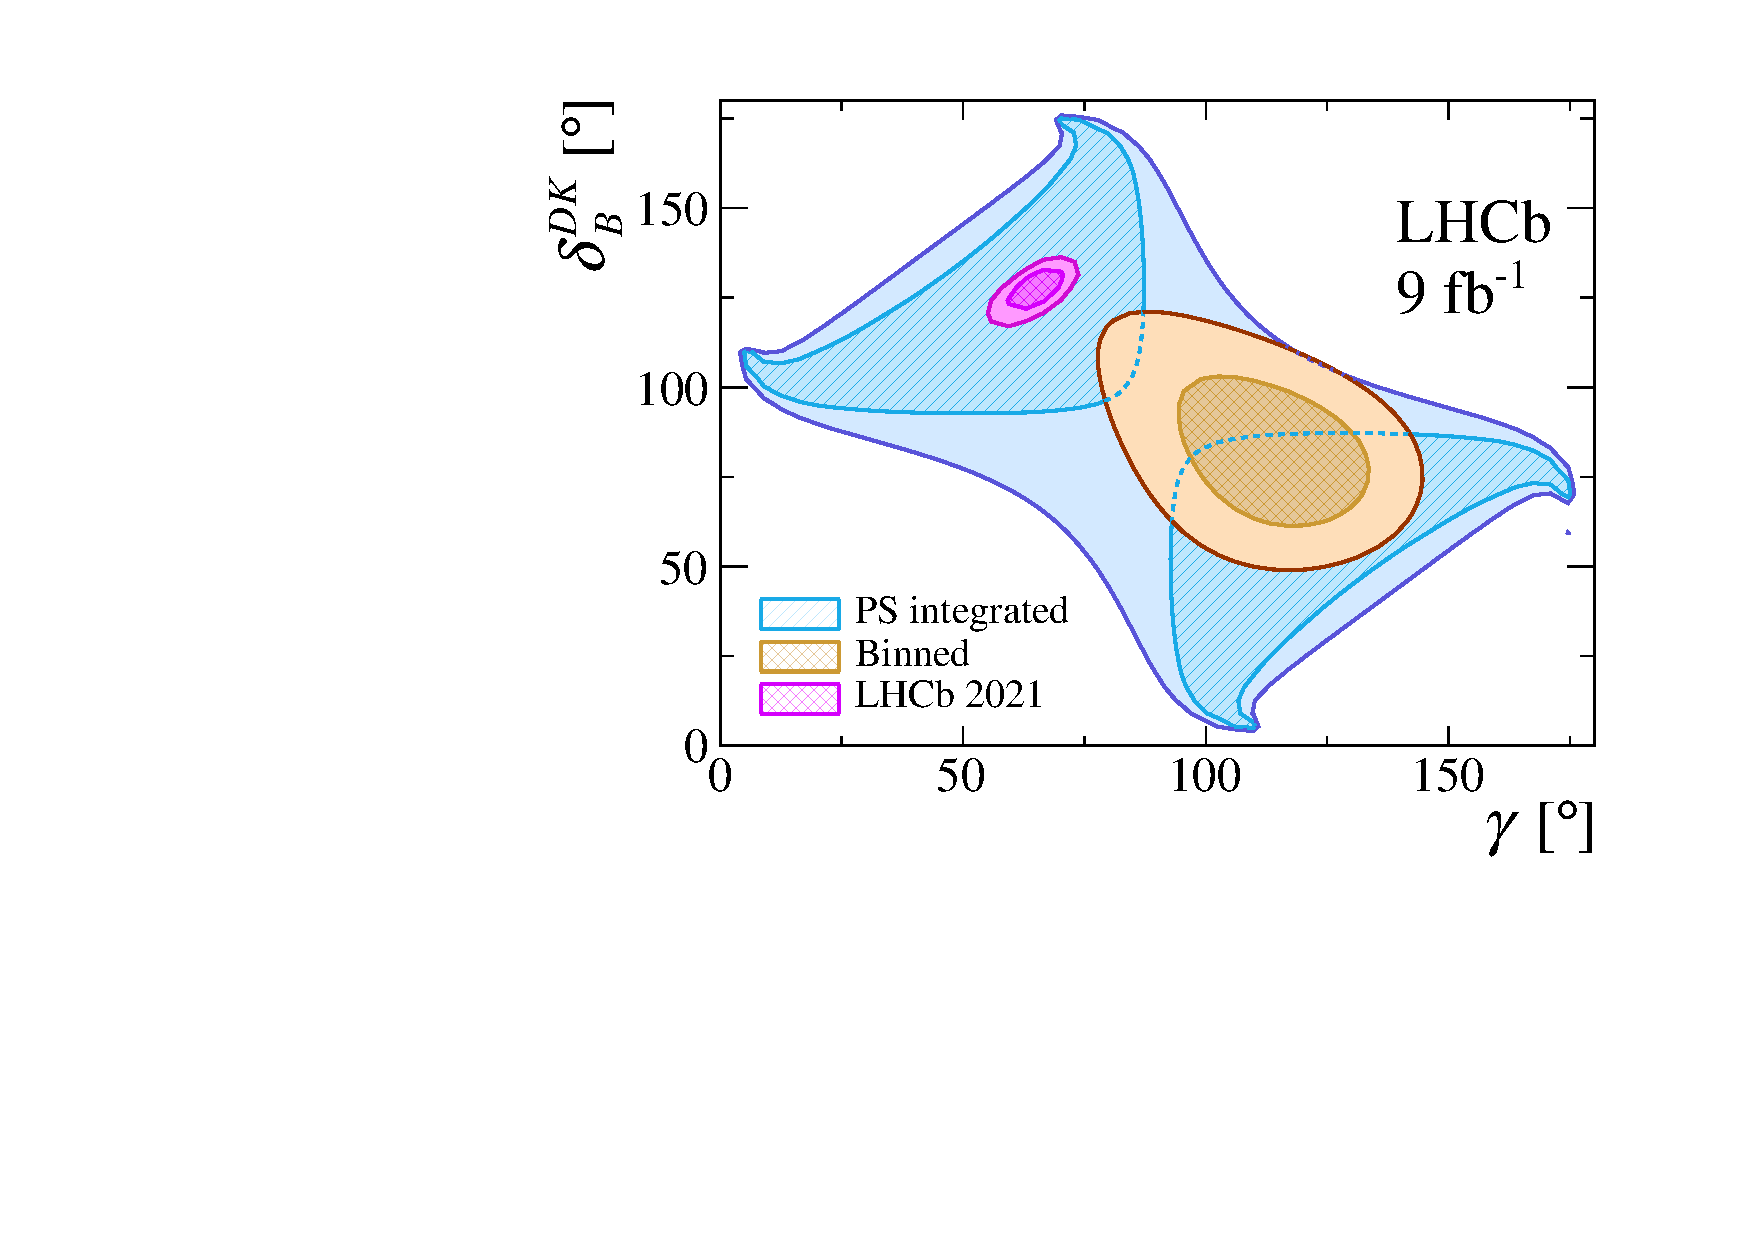
\includegraphics[width=1\textwidth]{Plots/gammacharm_lhcb_KKpipi_GLW_KKpipi_GGSZ_lhcb_2020_beauty_and_charm_g_d_dk.pdf}
    \end{subfigure}
    \vspace{-0.5cm}
    \caption*{\tiny\href{https://link.springer.com/article/10.1140/epjc/s10052-023-11560-5}{Eur. Phys. J. C \textbf{83}, 547 (2023)}}
  \end{figure}
  \vspace{-0.5cm}
  \begin{center}
    {\large These results are \underline{model dependent}, and will be updated once BESIII strong-phase inputs are available}
  \end{center}
\end{frame}

\section{Neutral \texorpdfstring{$B$}{B} decays}
\begin{frame}{Neutral $B$ decays}
  \begin{center}
  {\Large This method works analogously with neutral $B$ decays:}\\~\\
  {\large LHCb-PAPER-2023-009 (in preparation)\quad \colorbox{lime}{New results!}}\\
  \end{center}
  \vspace{0.5cm}
  \begin{figure}[H]
    \centering
    \begin{fmffile}{fgraph/fgraph_B02DKst_Kst2Kpi}
      \setlength{\unitlength}{0.7cm}
      \begin{fmfgraph*}(6,4)
        \fmfstraight
        \fmfleft{i1}
        \fmfv{decor.shape=circle,decor.filled=shaded,decor.size=0.2w,label=$B^0$,label.angle=180,label.dist=0.5cm}{i1}
        \fmfright{o1,o2,o3,g1,o4,o5}
        \fmflabel{$\pi^-$}{o1}
        \fmflabel{$\pi^+$}{o2}
        \fmflabel{$K_S^0$}{o3}
        \fmflabel{$\pi^-$}{o4}
        \fmflabel{$K^+$}{o5}
        \fmf{plain,tension=2.0}{i1,v1}
        \fmfv{decor.shape=circle,decor.filled=shaded,decor.size=0.15w,label=\small$K^*(892)^0$,label.angle=100,label.dist=1.7cm}{v1}
        \fmf{plain}{v1,o1}
        \fmf{plain}{v1,o2}
        \fmf{plain}{v1,o3}
        \fmf{dashes,tension=2.0}{i1,v2}
        \fmfv{decor.shape=circle,decor.filled=shaded,decor.size=0.15w,label=\footnotesize$D^0$,label.angle=-100,label.dist=1.6cm}{v2}
        \fmf{phantom}{v2,g1}
        \fmf{plain}{v2,o4}
        \fmf{plain}{v2,o5}
      \end{fmfgraph*}
    \end{fmffile}
  \end{figure}
  \vspace{0.5cm}
  \begin{center}
    {\Large $B^0\to(K_S^0h^+h^-)_D(K^+\pi^-)_{K^*}$}
  \end{center}
  \begin{center}
  {\large This results supersedes that of \href{https://link.springer.com/article/10.1007/JHEP08(2016)137}{JHEP \textbf{08} (2016) 137}}
  \end{center}
\end{frame}

\begin{frame}{Neutral $B$ decays}
  \begin{figure}
    \begin{subfigure}{0.45\textwidth}
      \centering
      \begin{overpic}[percent,height=4.0cm]{Plots/Kspp_LL_GF_B0toDKst.pdf}
        \put(58,32.7){\tiny Preliminary}
      \end{overpic}
      \caption*{LL}
    \end{subfigure}%
    \begin{subfigure}{0.45\textwidth}
      \centering
      \begin{overpic}[percent,height=4.0cm]{Plots/Kspp_DD_GF_B0toDKst.pdf}
        \put(58,32.7){\tiny Preliminary}
      \end{overpic}
      \caption*{DD}
    \end{subfigure}
    \vspace{-0.5cm}
    \caption*{\tiny LHCb-PAPER-2023-009}
  \end{figure}
  \vspace{-0.5cm}
  \begin{itemize}
    \setlength\itemsep{0.5em}
    \item{Two separate selections of $K^0_S$:}
    \begin{itemize}
      \item{LL (long tracks): $K^0_S$ decays in the VELO}
      \item{DD (downstream tracks): $K^0_S$ decays downstream of the VELO}
    \end{itemize}
    \item{$B^0\to DK^{*0}$ candidates with $D\to K_S^0\pi^+\pi^-$ ($D\to K_S^0K^+K^-$):}
    \begin{itemize}
      \item{LL: $102 \pm 17$ ($12 \pm 6$)}
      \item{DD: $288 \pm 25$ ($32 \pm 8$)}
    \end{itemize}
  \end{itemize}
\end{frame}

\begin{frame}{Neutral $B$ decays}
  \begin{figure}
    \begin{overpic}[percent,height=5.0cm]{Plots/CPFitAsymmetry_B0toDKst.pdf}
      \put(34.5,39.5){\tiny Preliminary}
    \end{overpic}
    \vspace{-0.2cm}
    \caption*{\tiny LHCb-PAPER-2023-009}
  \end{figure}
  \begin{itemize}
    \setlength\itemsep{0.5em}
    \item{Non-zero bin asymmetries are observed:}
    \begin{itemize}
      \item{\underline{Large} asymmetries are seen between $B^0$ ($\bar{B^0}$) bin pairs}
      \item{No CPV is expected in $B^0_s$ decays, and no such CPV is observed}
    \end{itemize}
    \item[]{\phantom{Asymmetries differ in size and magnitude across bins of phase space}}
  \end{itemize}
\end{frame}

\begin{frame}{Neutral $B$ decays}
  \begin{figure}
    \begin{overpic}[percent,height=5.0cm]{Plots/Asymmetry_B0toDKst.pdf}
      \put(56.5,9.5){\tiny Preliminary}
    \end{overpic}
    \vspace{-0.2cm}
    \caption*{\tiny LHCb-PAPER-2023-009}
  \end{figure}
  \begin{itemize}
    \setlength\itemsep{0.5em}
    \item{Non-zero bin asymmetries are observed:}
    \begin{itemize}
      \item{\underline{Large} asymmetries are seen between $B^0$ ($\bar{B^0}$) bin pairs}
      \item{No CPV is expected in $B^0_s$ decays, and no such CPV is observed}
    \end{itemize}
    \item{Asymmetries differ in size and magnitude across bins of phase space}
  \end{itemize}
\end{frame}

\begin{frame}{Neutral $B$ decays}
  \begin{figure}
    \centering
    \begin{subfigure}{0.45\textwidth}
      \centering
      \begin{overpic}[percent,height=4.0cm]{Plots/cp_contours_B0toDKst.pdf}
        \put(67,67.5){\tiny Preliminary}
      \end{overpic}
    \end{subfigure}%
    \begin{subfigure}{0.45\textwidth}
      \centering
      \begin{overpic}[percent,height=4.0cm]{Plots/B0ToDKStar_GGSZ_g_db_B0toDKst.pdf}
        \put(70.5,50){\tiny Preliminary}
      \end{overpic}
    \end{subfigure}
    \vspace{-0.2cm}
    \caption*{\tiny LHCb-PAPER-2023-009}
  \end{figure}
  \vspace{-0.5cm}
  \begin{itemize}
    \setlength\itemsep{0.5em}
    \item{Measured $C\!P$-violating observables:}
    \begin{center}
      $x_\pm\equiv r_{B^0}\cos(\delta_{B^0} \pm \gamma)$ and $y_\pm\equiv r_{B^0}\sin(\delta_{B^0} \pm \gamma)$
    \end{center}
    \item{Measured value of $\gamma$ is consistent with world average:}
    \begin{itemize}
      \item{$\gamma = (49 \pm 20)^\circ$}
      \item{$\delta_{B^0} = (236 \pm 19)^\circ$}
      \item{$r_{B^0} = 0.27 \pm 0.07$}
    \end{itemize}
  \end{itemize}
\end{frame}

\section{\texorpdfstring{$B$}{B} decays to excited \texorpdfstring{$D^*$}{Dst} final states}
\begin{frame}{$B$ decays to excited $D^*$ final states}
  \begin{center}
  {\Large $B^-\to D^*K^-$ decays are also a powerful probe of CPV:}\\~\\
  {\large LHCb-PAPER-2023-012 (in preparation)\quad \colorbox{lime}{New results!}}
  \end{center}
  \vspace{0.5cm}
  \begin{figure}[H]
    \centering
    \begin{subfigure}{0.45\textwidth}
      \centering
      \begin{fmffile}{fgraph/fgraph_BtoDstK_pi0}
        \setlength{\unitlength}{0.7cm}
        \begin{fmfgraph*}(4,3)
          \fmfstraight
          \fmfleft{i1}
          \fmfv{decor.shape=circle,decor.filled=shaded,decor.size=0.2w,label=$B^-$,label.angle=180,label.dist=0.5cm}{i1}
          \fmfright{o1,o2,o3}
          \fmflabel{$K^-$}{o1}
          \fmflabel{$\pi^0$}{o2}
          \fmflabel{$D$}{o3}
          \fmf{dashes,tension=1.5}{i1,v1}
          \fmfv{decor.shape=circle,decor.filled=shaded,decor.size=0.15w,label=\small$D^*$,label.angle=100,label.dist=0.5cm}{v1}
          \fmf{plain}{v1,o2}
          \fmf{plain}{v1,o3}
          \fmf{plain}{i1,o1}
        \end{fmfgraph*}
      \end{fmffile}
      \vspace{0.5cm}
      \caption*{$B^-\to[D\pi^0]_{D^*}K^-$}
    \end{subfigure}%
    \begin{subfigure}{0.45\textwidth}
      \centering
      \begin{fmffile}{fgraph/fgraph_BtoDstK_gamma}
        \setlength{\unitlength}{0.7cm}
        \begin{fmfgraph*}(4,3)
          \fmfstraight
          \fmfleft{i1}
          \fmfv{decor.shape=circle,decor.filled=shaded,decor.size=0.2w,label=$B^-$,label.angle=180,label.dist=0.5cm}{i1}
          \fmfright{o1,o2,o3}
          \fmflabel{$K^-$}{o1}
          \fmflabel{$\gamma$}{o2}
          \fmflabel{$D$}{o3}
          \fmf{dashes,tension=1.5}{i1,v1}
          \fmfv{decor.shape=circle,decor.filled=shaded,decor.size=0.15w,label=\small$D^*$,label.angle=100,label.dist=0.5cm}{v1}
          \fmf{plain}{v1,o2}
          \fmf{plain}{v1,o3}
          \fmf{plain}{i1,o1}
        \end{fmfgraph*}
      \end{fmffile}
      \vspace{0.5cm}
      \caption*{$B^-\to[D\gamma]_{D^*}K^-$}
    \end{subfigure}
  \end{figure}
  \vspace{-0.5cm}
  \begin{columns}
    \begin{column}{0.5\textwidth}
      \begin{center}
        $\mathcal{A}(B^-)\propto\mathcal{A}(D^0) + r_Be^{i(\delta_B - \gamma)}\mathcal{A}(\bar{D^0})$
      \end{center}
    \end{column}
    \begin{column}{0.5\textwidth}
      \begin{center}
        $\mathcal{A}(B^-)\propto\mathcal{A}(D^0) - r_Be^{i(\delta_B - \gamma)}\mathcal{A}(\bar{D^0})$
      \end{center}
    \end{column}
  \end{columns}
  \begin{center}
    The relative sign swap, due to the phase difference of $\pi$ between $\pi^0$ and $\gamma$,  results in \underline{opposite} $C\!P$ asymmetries between $D^*\to D\pi^0$ and $D^*\to D\gamma$
  \end{center}
\end{frame}

\begin{frame}{$B$ decays to excited $D^*$ final states}
  \begin{figure}
    \centering
    \begin{subfigure}{0.5\textwidth}
      \centering
      \begin{overpic}[percent,width=0.8\textwidth]{Plots/massfitPage_canvas_pi0_d2kspipi_b2dpi_LL_merge_BtoDstpi.pdf}
        \put(59,82){\tiny Preliminary}
        \put(36,48){\vector(-1.0,1.9){14}}
        \put(36,48){\vector(-1.0,-1.5){14}}
        \put(37,47.5){\scriptsize Signal peak}
      \end{overpic}
      \caption*{$D^*\to D\pi^0$}
    \end{subfigure}%
    \begin{subfigure}{0.5\textwidth}
      \centering
      \begin{overpic}[percent,width=0.8\textwidth]{Plots/massfitPage_canvas_gamma_d2kspipi_b2dpi_LL_merge_BtoDstpi.pdf}
        \put(59,82){\tiny Preliminary}
        \put(26,53){\vector(1.0,30.0){0.5}}
        \put(26,53){\vector(1.0,-1.0){30}}
        \put(0,50){\scriptsize Signal peak}
      \end{overpic}
      \caption{$D^*\to D\gamma$}
    \end{subfigure}
    \vspace{-0.2cm}
    \caption*{\tiny LHCb-PAPER-2023-012}
  \end{figure}
\end{frame}

\begin{frame}{$B$ decays to excited $D^*$ final states}
  \begin{figure}
    \begin{overpic}[percent,height=5.0cm]{Plots/histCPVnewd2kspipib2dk_BtoDstK.png}
      \put(57.5,32){\tiny Preliminary}
    \end{overpic}
    \vspace{-0.4cm}
    \caption*{\tiny LHCb-PAPER-2023-012}
  \end{figure}
  \vspace{-0.5cm}
  \begin{itemize}
    \setlength\itemsep{0.5em}
    \item{Good agreement between individual bin asymmetries and the combined $C\!P$ fit}
    \item{Bin asymmetries between $D^*\to D\pi^0$ and $D^*\to D\gamma$ are generally \underline{opposite} in sign}
  \end{itemize}
\end{frame}

\begin{frame}{$B$ decays to excited $D^*$ final states}
  \begin{figure}
    \centering
    \begin{subfigure}{0.5\textwidth}
      \centering
      \begin{overpic}[percent,height=5.0cm]{Plots/xyfinalres_BtoDstK.pdf}
        \put(27,69){\tiny Preliminary}
      \end{overpic}
    \end{subfigure}%
    \begin{subfigure}{0.5\textwidth}
      \centering
      \begin{overpic}[percent,height=4.3cm]{Plots/cartesian_cartesian1_g_r_dk_BtoDstK.pdf}
        \put(72,54){\tiny Preliminary}
      \end{overpic}
    \end{subfigure}
    \vspace{-0.8cm}
    \caption*{\tiny LHCb-PAPER-2023-012}
  \end{figure}
  \vspace{-0.7cm}
  \begin{center}
    These results provide strong constraints on $\gamma$:
  \end{center}
  \vspace{-0.2cm}
  \begin{itemize}
  \item{$\gamma = (69 \pm 14)^\circ$}
  \item{$\delta_B^{D^*K} = (311 \pm 15)^\circ$}
  \item{$r_B^{D^*K} = 0.15 \pm 0.03$}
  \end{itemize}
\end{frame}

\section{Summary and future prospects}
\begin{frame}{Summary and future prospects}
  \vspace{0.0cm}
  {\Large In summary:}
  \vspace{0.3cm}
  \begin{enumerate}
    \setlength\itemsep{1.0em}
    \item{LHCb performed several measurements of $\gamma$, using a set of complementary $B$ and $D^{(*)}$ decay combinations}
    \item{Phase-space binned analyses using the golden mode $D\to K_S^0\pi^+\pi^-$ provide the most powerful constraints for our $\gamma$ combination}
    \item{A binned measurement with the channel $B^\pm\to[K^+K^-\pi^+\pi^-]_DK^\pm$ has been performed for the first time}
    \begin{itemize}
      \item{Need external inputs for charm strong-phases from BESIII}
    \end{itemize}
    \item{I have also presented two new model-independent measurements:}
    \begin{itemize}
      \item{$B^0\to DK^{*0}$ with $K^{*0}\to K^+\pi^-$}
      \item{$B^\pm\to D^{*}h^\pm$ with $D^*\to D\pi^0$ and $D\gamma$}
    \end{itemize}
  \end{enumerate}
\end{frame}

\begin{frame}{Summary and future prospects}
  \vspace{0.0cm}
  {\Large Future prospects:}
  \vspace{0.3cm}
  \begin{enumerate}
    \setlength\itemsep{1.0em}
    \item{The measurements I have presented today will make valuable improvements to future $\gamma$ combinations}
    \item{Measurements are still dominated by statistical uncertainties, and are expected to reduce significantly at the end of Run 3}
    \item{We expect more time-dependent results, such as $B_s^0\to D_s^-K^+$ with Run 2, that will be interesting to compare with results from $B^\pm$/$B^0$}
    \end{enumerate}
    \vspace{1.0cm}
  \begin{center}
    {\huge Thanks for your attention!}
  \end{center}
\end{frame}

\end{document}
